\documentclass[10pt,letterpaper]{article}
\usepackage[top=0.85in,left=2.75in,footskip=0.75in]{geometry}

% amsmath and amssymb packages, useful for mathematical formulas and symbols
\usepackage{amsmath,amssymb}

\usepackage{graphicx}
\usepackage{booktabs}

% Use adjustwidth environment to exceed column width (see example table in text)
\usepackage{changepage}
\usepackage{tabularx}

% Use Unicode characters when possible
\usepackage{inputenc}

% textcomp package and marvosym package for additional characters
\usepackage{textcomp,marvosym}

% cite package, to clean up citations in the main text. Do not remove.
\usepackage{cite}

% Use nameref to cite supporting information files (see Supporting Information section for more info)
\usepackage{nameref,hyperref}

% line numbers
\usepackage[right]{lineno}

\usepackage{tikz}

% ligatures disabled
\usepackage{microtype}
\DisableLigatures[f]{encoding = *, family = * }


% array package and thick rules for tables
\usepackage{array}

\usepackage{algorithm}
\usepackage{algpseudocode}

\usepackage{float}
\usepackage{timestamp}
\usepackage{xfrac}
\usepackage{mathtools}

%% Include all macros below

\newcommand{\lorem}{{\bf LOREM}}
\newcommand{\ipsum}{{\bf IPSUM}}

%% END MACROS SECTION
\newcommand{\R}{\mathbb{R}}

\begin{document}
\vspace*{0.2in}

% Title must be 250 characters or less.
\begin{flushleft}
{\Large
\textbf\newline{A Monte Carlo method to estimate cell population heterogeneity}
}
\newline
\\
Ben Lambert\textsuperscript{1,2}*,
David J. Gavaghan\textsuperscript{3},
Simon Tavener\textsuperscript{4}.
\\
\bigskip
\textbf{1} Department of Zoology, University of Oxford, Oxford, Oxfordshire, U.K.
\\
\textbf{2} MRC Centre for Global Infectious Disease Analysis, School of Public Health, Imperial College London, London W2 1PG, UK.
\\
\textbf{3} Department of Computer Science, University of Oxford, Oxford, U.K.
\\
\textbf{4} Department of Mathematics, Colorado State University, Fort Collins, CO 80523, U.S.A.
\\
\bigskip

% Use the asterisk to denote corresponding authorship and provide email address in note below.
*ben.c.lambert@gmail.com.

\end{flushleft}

\hfill Revision date \& time: \timestamp
\bigskip


% Please keep the abstract below 300 words
%%%%%%%%%%%%%%%%%%%%%%%%%%%%%%%%%%%%%%%%%%%%%%%%%%%%%%%%%%%%%%%%%%%%%%%%%%%%%%%%%%%%%%%%%%%%%%%%%%%%%%%%%%%%%%%%%%%%%%%%                                                                                                                  %                                                                                                                      %
%       ABSTRACT                                                                                                       %
%                                                                                                                      %
%%%%%%%%%%%%%%%%%%%%%%%%%%%%%%%%%%%%%%%%%%%%%%%%%%%%%%%%%%%%%%%%%%%%%%%%%%%%%%%%%%%%%%%%%%%%%%%%%%%%%%%%%%%%%%%%%%%%%%%%

% The Abstract of the paper should be succinct; it must not exceed 300 words. Authors should mention the techniques used without going into methodological detail and should summarize the most important results.

% While the Abstract is conceptually divided into three sections (Background, Methodology/Principal Findings, and Conclusions/Significance), do not apply these distinct headings to the Abstract within the article file.

% Do not include any citations. Avoid specialist abbreviations.
\newpage
\linenumbers
\section{Abstract}
Variation is characteristic of all living systems. Laboratory techniques such as flow cytometry can probe individual cells and, after decades of experimentation, it is clear that even members of seemingly homogeneous cell populations can exhibit differences. To understand whether this variation is biologically meaningful, it is essential to discern its source. Mathematical models of biological systems are tools that can be used to investigate causes of cell-to-cell variation. From mathematical analysis and simulation of these models, biological hypotheses can be posed and investigated, then parameter inference can determine which of these is most compatible with experimental data. Data from laboratory experiments often takes the form of ``snapshots" representing distributions of cellular properties at different points in times, rather than individual cell trajectories. This data is not straightforward to fit using hierarchical Bayesian methods since it requires inferring the identities of the groups to which individual cells belong. Here, we introduce a computational sampling method we call ``Contour Monte Carlo" for estimating mathematical model parameters from snapshot distributions which is straightforward to implement and does not require explicitly assigning cells to categories. Our method is most applicable to systems where the dominant source of uncertainty is heterogeneity in cellular processes rather than experimental measurement error which, due to the increasingly finescale resolution of laboratory techniques, may be the case for a wide class of systems. In this paper, we illustrate the use of our method by quantifying cellular variation for three biological systems of interest and provide code in the form of a Julia notebook which allows others to apply this approach to their problem.

\section{Introduction}
Variation, as opposed to homogeneity, is the rule rather than exception in biology. Indeed, without variation, biology as a discipline would not exist, since as evolutionary biologist JBS Haldane wrote, variation is the ``raw material" of evolution. The Red Queen Hypothesis asserts organisms must continually evolve in order to survive when pitted against other - also evolving - organisms \cite{ridley1994red}. A corollary of this hypothesis is that multicellular organisms should evolve cellular phenotypic heterogeneity to allow faster adaptation to changing environments, which may explain the observed variation in a range of biological systems \cite{fraser2009chance}. Whilst cell population variation can confer evolutionary advantages, it can be costly in other circumstances. In biotechnological processes, heterogeneity in cellular function can reduce yields of biochemical products \cite{delvigne2014metabolic}. In human biology, variation across cells can enable pathologies to develop; it can also frustrate treatment of illness because key subpopulations are missed by medical interventions that target ``average'' cell properties. For example, cellular heterogeneity helps some cancerous tumours to persist \cite{gatenby2007cellular} and can make tumours more likely to evolve resistance to chemotherapies \cite{altrock2015mathematics}. To discern whether observed variation is benign or requires remedy, methods of analysis are needed that can quantify and help to understand its source.

Mathematical models are essential tools for understanding cellular systems, whose emergent properties are the result of a nexus of interactions between actors. Perhaps the simplest flavour of mathematical model used in biological systems is an ordinary differential equation (ODE) that aggregates individual actors into compartments according to structure or function, and seeks to model the mean behaviour of each compartment. Data from population-averaged experimental assays can determine whether such models faithfully reproduce system behaviours and can be used to understand the structure of complex metabolic, signalling and transcriptional networks. The worth of such ``population average'' ODE models depends on whether averages mask substantial differences in individual behaviour \cite{altschuler2010cellular}. In some cases, differences in cellular protein abundances due to biochemical ``noise" are not biologically meaningful \cite{elowitz2002stochastic} and the system is well described by average cell behaviour. In others, there are functional consequences. For example, a laboratory study demonstrated that subpopulations of clonally-derived hematopoietic progenitor cells with low expression of a stem cell marker, diverged into a separate blood lineage from those with high expression \cite{chang2008transcriptome}.

Many modelling frameworks are available to describe cell population heterogeneity, with each posing different challenges for parameter inference. A recent review is presented in \cite{waldherr2018estimation}. These approaches include modelling biochemical processes stochastically, where properties of ensembles of cells are represented by probability distributions that evolve according to chemical master equations. See \cite{erban2007practical} for a tutorial on stochastic simulation of reaction diffusion processes. Alternatively, population balance equations (PBEs) are typically partial integro-differential equations that determine the dynamics of the ``number density" of differing cell types. In PBEs, cell properties are represented as points in $\mathbb{R}^n$, with each dimension corresponding to a different attribute. These attributes include parameters controlling cell life - for example, their rate of death and division, which vary according to a cell's location in this ``attribute'' space. These functional differences control the rate at which cells progress through life, which is represented by a ``flow'' of cells from certain areas of attribute space to others - like chemicals diffusing down a concentration gradient. With PBEs, observed variation at a point in time is due to the initial spread of cells across attribute space coupled with the differing dynamics of cells in different areas of this space. See \cite{ramkrishna2014population} for an introduction to PBEs.

Here, we suppose heterogeneity in quantities of interest across cells is generated by idiosyncratic variation in the rates of cellular processes. The modelling approach we follow is similar to that of \cite{dixit2018maximum} and is based on an ODE framework. In our model, each cell evolves according to an ODE, with its progression directed by parameters whose value varies between cells. To our knowledge, this flavour of model is unnamed, so, for sake of reference, we call them ``heterogenous ODE" models (HODEs). In HODEs, the aim of inference is to estimate distributions of parameter values across cells consistent with observations. A benefit of using HODEs is that these models are computationally straightforward to simulate and, arguably, simpler to parameterise than PBEs. By using HODEs, we assume that most observed variation comes from differences in biological processes across cells, not inherent stochasticity in biochemical reactions within cells as is assumed when employing stochastic simulations algorithms.

Inference for HODEs is problematic due, partly, to the experimental hurdles involved with generating data of sufficient standard. Unlike models which represent a population by a single scalar ODE, since HODEs are individual-based, they ideally require individual cell data for estimation. A widely-used method for generating such data is flow cytometry, where a large number of cells are streamed individually through a laser beam, and, for example, the concentrations of fluorescently-labelled proteins are measured \cite{telford2012flow}. Other experimental techniques, including Western blotting and cytometric fluorescence microscopy, can also generate single cell measurements \cite{hughes2014single,hasenauer2011identification}. These experimental methods are all, however, destructive, meaning individual cells are sacrificed during measurement, and observations at each time point hence represent \emph{``snapshots"} of the underlying population \cite{hasenauer2011identification}. These snapshots can be described by histograms \cite{dixit2018maximum} or density functions \cite{waldherr2018estimation} fit to measurements of quantities of interest. Since HODEs assume the state of each cell evolves continuously over time, experimental data tracing individual cell trajectories through time constitutes a richer data resource. \textcolor{blue}{Fluorescent Recovery After Photo-bleaching (FRAP) is one such method, which follows the time-dependent response of cells after an initial bleaching \cite{karlsson2015nonlinear}. Methods exists, broadly under the banner of ``nonlinear mixed effects models'', which use cell trajectories -- individual time series of cellular quantities -- to estimate both cellular variation and qualities of measurement noise. See, for example, \cite{karlsson2015nonlinear,zechner2014scalable,dharmarajan2019simple}.} The demands of obtaining such data are, however, higher and typically involve either tracking individual cells through imaging methods \cite{hilsenbeck2016software}, or trapping cells in a spatial position where they can be monitored over time \cite{fritzsch2012single}. These techniques impose severe restrictions on experimental practices meaning they cannot be used in many circumstances, including for online monitoring of biotechnological processes or analysis of \textit{in vivo} studies. \textcolor{blue}{``Snapshot''} data continues to play an important role for determining cell level variability in many applications \textcolor{blue}{and in this paper we restrict analysis to only such data.}

By fitting HODES to snapshot data, cellular variability can be estimated and a number of approaches have been proposed for doing so. In HODEs, parameter values vary across cells according to a to-be-determined probability distribution, and the solution to the inverse problem requires solving the cell-specific ODE system many times for each individual. The count of cells in experiments typically exceeds $\sim10^4$ \cite{hasenauer2011identification}, so approaches where the computational burden scales with this count are usually infeasible. To avoid this burden, some approaches fit probability densities to raw snapshot data and use these densities, rather than raw data, for estimation \cite{hasenauer2011identification,hasenauer2014ode,loos2018hierarchical,dixit2018maximum}. We follow this approach here. We now briefly describe the existing approaches for using HODE models to estimate cell population heterogeneity. Hasenauer et al. (2011) present a Bayesian approach to inference for HODEs, which models the input parameter space using an ansatz of a mixture of densities of chosen types. The authors then use their method to reproduce population substructure on synthetic data generated from a model of tumour necrosis factor stimulus. Hasenauer et al. (2014) use mixture models to model subpopulation structure in snapshot data with multiple-start local optimisation employed to maximise the non-convex likelihood, which they then apply to synthetic and real data from signalling pathway models. Loos et al. (2018) also use mixture models to represent subpopulation structure and use maximum likelihood to estimate both within- and between-subpopulation variability, which permits fitting to multivariate output distributions with complex correlation structures. Dixit et al. (2018) assign observations into discrete bins, then choose likelihood distributions according to the maximum entropy criterion, which they then use to estimate cell variability within a Bayesian framework.

Our framework is Bayesian although it is distinct from the approach used to fit many dynamic models, since we assume output variation arises from parameter heterogeneity across cells, with no contribution from measurement noise. The approach is, hence, most suitable when measurement error is minimal. Additionally, our approach is suitable only for underdetermined models \textcolor{blue}{- which we define as the case where there are fewer output quantities of interest than parameters. Since the generation of snapshots is expensive, it is often the case that fewer observables are recorded than parameters. Hence, we believe that this restriction does not present particular issue to the generalisability of our approach.} Our method is a two-step Monte Carlo approach, which, for reasons described in \S \ref{sec:method}, we call ``Contour Monte Carlo'' (CMC). Unlike many existing methods, CMC is straightforward to implement and does not require extensive computation time. In CMC, prior probability distributions are used in place of ansatz densities. It also does not require the number of cell clusters be chosen beforehand, rather, subpopulations emerge as modes in the posterior parameter distributions. Like \cite{loos2018hierarchical}, CMC can fit multivariate snapshot data and unlike \cite{dixit2018maximum}, does not use discrete bins to model continuous data. As more experimental techniques elucidating single cell behaviour are developed, interest in models describing measurement snapshots should follow. We argue that due to its simplicity and generality, CMC can be used to perform inference on the proliferation of rich single cell data and, thus, is a useful addition to the modeller's toolkit.


\underline{Outline of the paper}: In \S \ref{sec:method}, we describe our probabilistic model of the inverse problem and detail the CMC algorithm for generating samples from the posterior parameter distribution. In \S \ref{sec:results}, we use CMC to estimate cell population heterogeneity in three systems of biological interest.



\section{Method}\label{sec:method}
In this section, we first develop a probabilistic framework that describes our inverse problem, before introducing the CMC algorithm in pseudocode (Algorithm \ref{alg:cmc}). We also detail the workflow we have found helpful in using CMC to analyse cell snapshot data (Figure \ref{fig:workflow}), and suggest practical remedies to issues commonly encountered while using this approach. A glossary of variable names used in this paper is included as Table \ref{tab:variable_glossary}.

Experimental methods such as flow cytometry measure single cell characteristics at a given time. Cells are typically destroyed by the measurement process, so the data consists of cross-sections or ``snapshots'' of sampled individuals from the population, rather than providing time series for each individual cell. The contrast between these two very different scenarios is highlighted in Figure \ref{fig:time_series_v_snapshots}. The cells at time $t_k$ are not the same as those at time $t_{k-1}$ and even if they are, there is no way of associating a particular cell at time $t_k$ with the same cell at time $t_{k-1}$. In other words, there is no sense of a ``trajectory'' of a specific cell, or of multiple observations assigned to a single cell.


\begin{figure}[H]
  \centerline{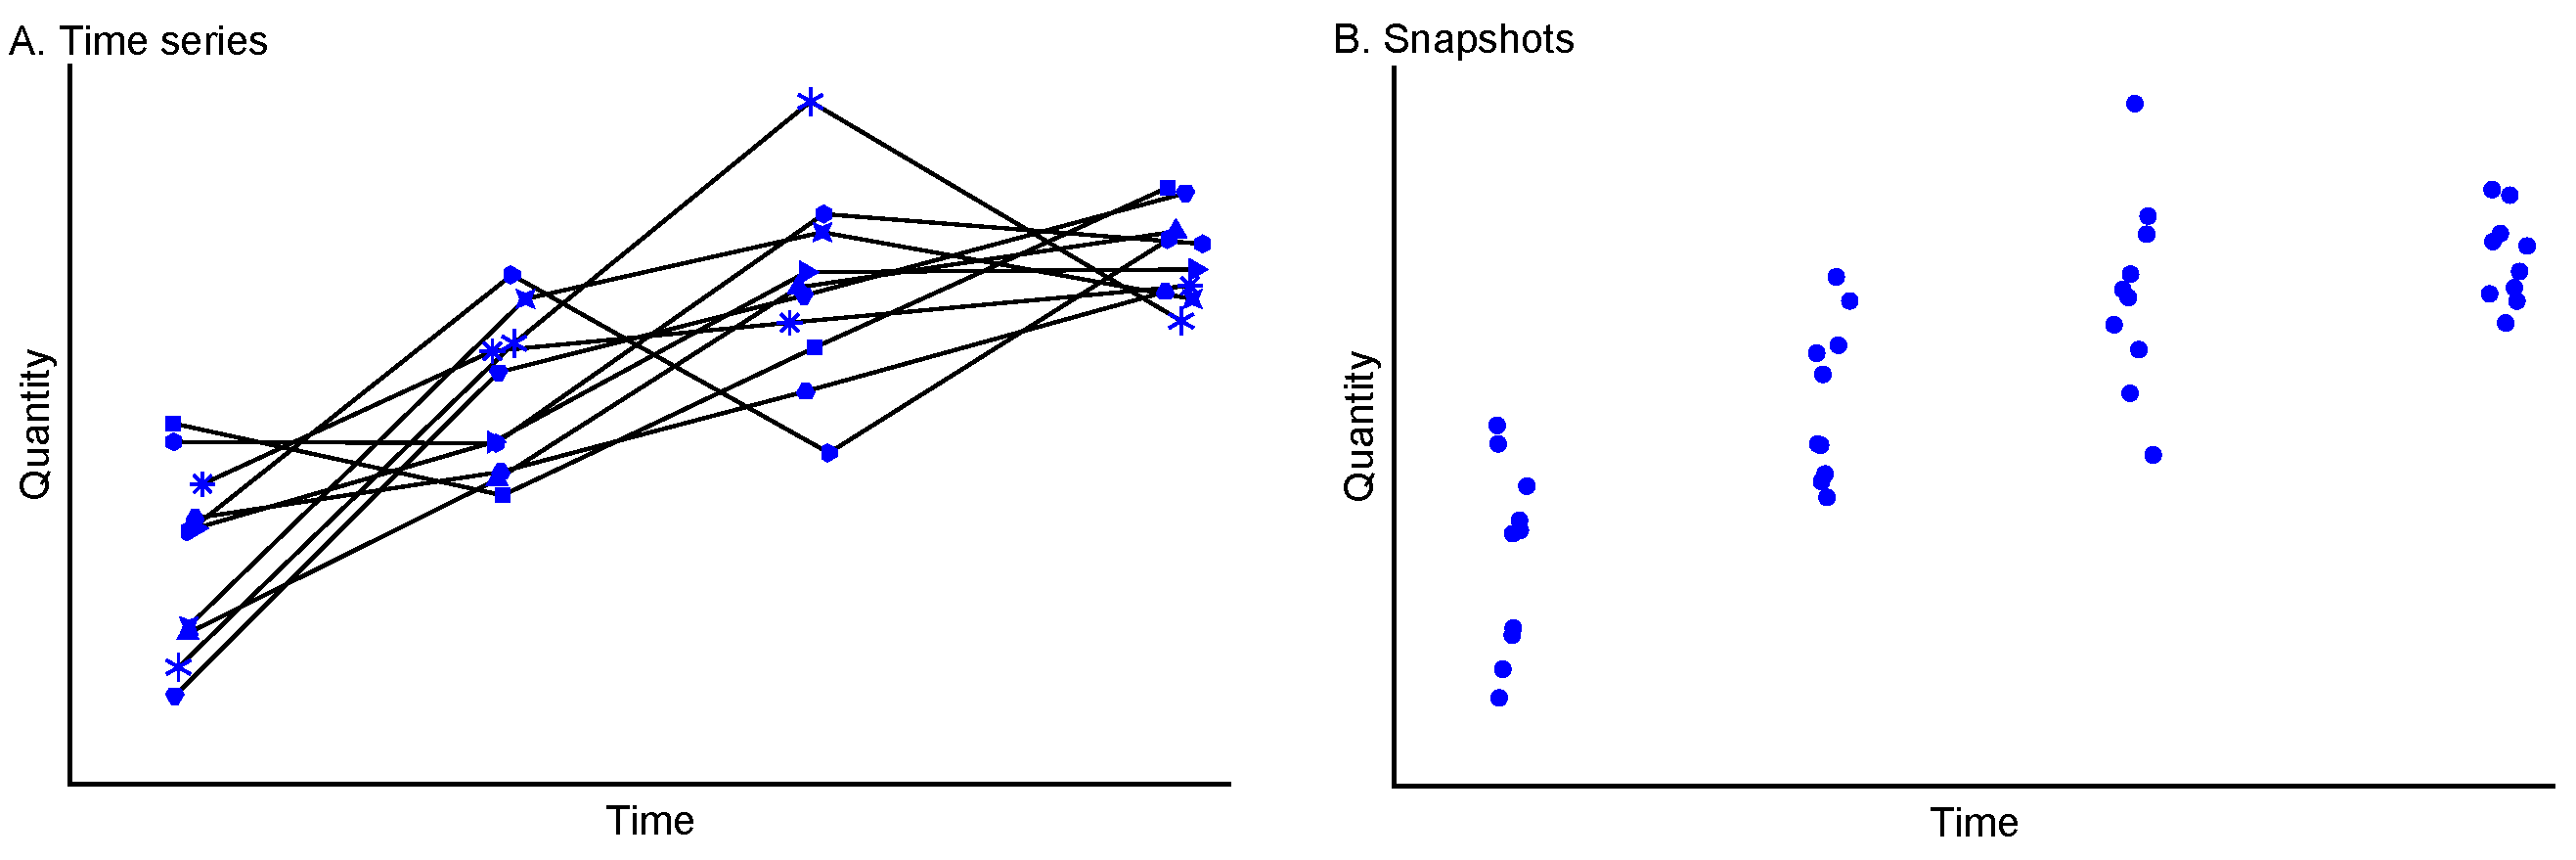
\includegraphics[width=\textwidth]{../figures/time_series_v_snapshots.pdf}}
  \caption{\textbf{Data typical of single cell experiments. (A) Time series data. (B) Snapshot data.} In A, note cell identities are retained at each measurement time (indicated by individual plot markers), whereas in the snapshot data in B, either this information is lost, or more often, cells are destroyed by the measurement process, and each observation corresponds to a distinct cell.}
  \label{fig:time_series_v_snapshots}
\end{figure}

We model the processes of an individual cell using a system of ordinary differential equations (ODEs), where each element of the system typically corresponds to the concentration of a particular species. Our initial value problem is,
%
\begin{equation}\label{eq:ode}
\begin{aligned}
\frac{d\boldsymbol{x}}{dt} &= \boldsymbol{f}(\boldsymbol{x}(t); \, \boldsymbol{\theta}), \quad \boldsymbol{f}: \R^k \times \R^p \mapsto \R^k, \\
\boldsymbol{x}(0) &= \boldsymbol{x}_0.
\end{aligned}
\end{equation}
%
Note that in most circumstances, the initial state of the system, $\boldsymbol{x}(0)$, is unknown, and it can be convenient to include these as elements of $\boldsymbol{\theta}$ to be estimated.

\subsection{Snapshot data}
We assume the variation in snapshots arises due to heterogeneity in the underlying parameters, $\boldsymbol{\theta}$, across cells. Therefore, the evolution of the underlying state of cell $i$ is described by an idiosyncratic ODE,
%
\begin{equation} \label{eq:ode_i}
\begin{aligned}
\frac{d\boldsymbol{x}^{\{i\}}}{dt} &= \boldsymbol{f} \left( \boldsymbol{x}^{\{i\}}(t); \, \boldsymbol{\theta}^{\{i\}} \right),
                                      \quad \boldsymbol{f}: \R^k \times \R^p \mapsto \R^k, \\
\boldsymbol{x}^{\{i\}}(0) &= \boldsymbol{x}_0,
\end{aligned}
\end{equation}
where superscript $^{\{i\}}$ indicates the $i$th cell. The collection of such idiosyncratic ODEs across all cells is then referred to as the ``HODE model''.

The traditional (non-hierarchical) state-space approach to modelling dynamic systems supposes that measurement error introduces stochastic variation in the output (Figure \ref{fig:data_generation}A). Our approach, by contrast, assumes any variation in outputs is solely due to variation in parameter values between cells (Figure \ref{fig:data_generation}B). Whether the assumption of ``perfect'' measurements is reasonable depends on experimental details of the system under investigation, but we argue our method nevertheless provides a useful approximation in cases where the signal to noise ratio is high. Once again we emphasize that we are considering distributions of quantities of interest with no sense of specific individual trajectories, making a mixed effects modelling approach problematic.


\begin{figure}[H]
  \centerline{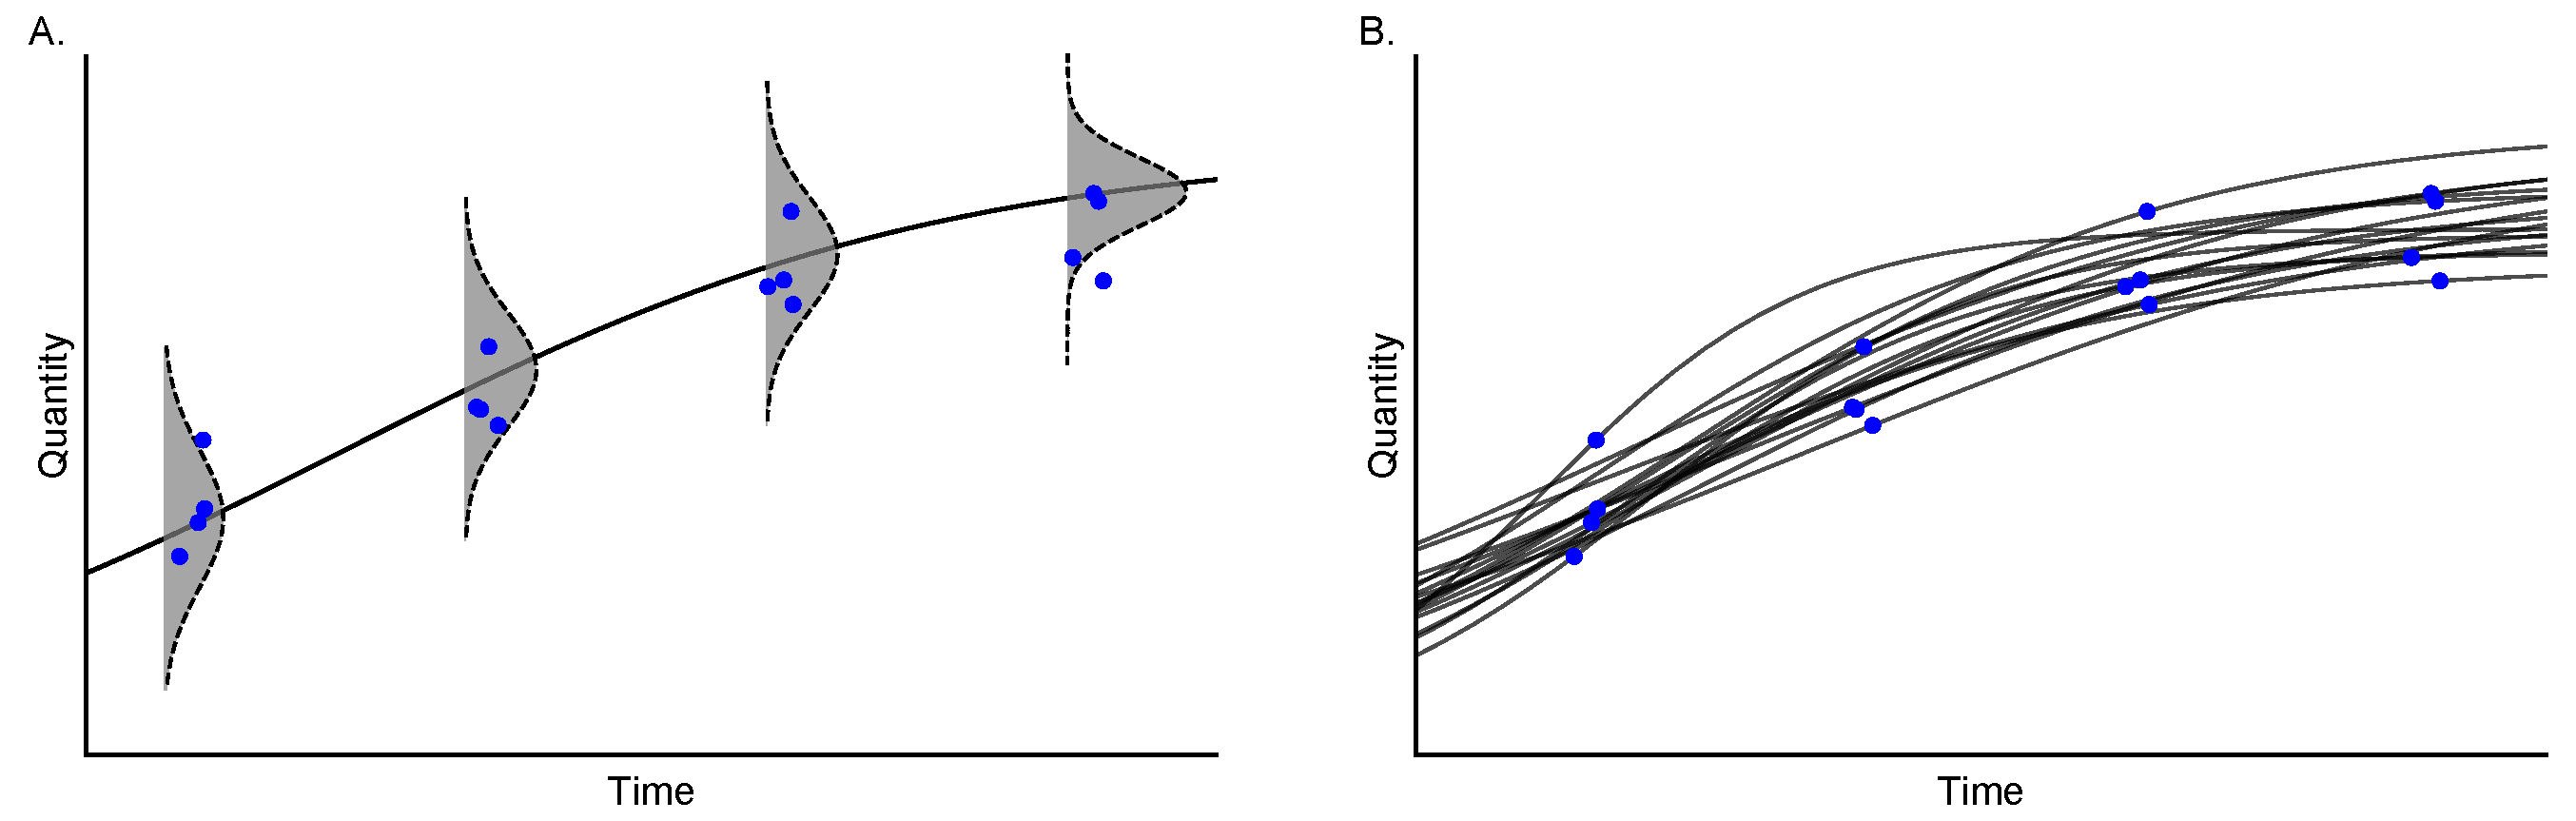
\includegraphics[width=\textwidth]{../figures/data_generation.pdf}}
  \caption{\textbf{Models of variation in observed outputs. (A) State-space model. (B) Parameter heterogeneity model.} (A) For non-hierarchical state-space models , there is a single ``true'' latent state, and observations result from an imperfect measurement process (grey histograms). (B) For models with parameter heterogeneity, the uncertainty is generated by differences in cellular processes (black lines) between cells. Note that, in both cases, individual cells are measured only once in their lifetime.}
  \label{fig:data_generation}
\end{figure}

In an experiment, quantities of interest (QOIs) are measured. Examples of QOIs include concentrations of compounds at different points in time, peak voltages across cell membranes during an action potential, or measurements of cell volume. Here, we suppose $m\geq 1$ QOIs are measured,
%
\begin{equation}
\boldsymbol{q}^\top = \left( q_1, q_2, \dots, q_m \right) \in \R^m,
\end{equation}
%
with $n_j$ observations of each quantity, $q_j$. Distinct QOIs, $q_j$, may correspond to different functionals of the solution at the same time or the same functional at different times. The observed data for QOI $q_j$ at the corresponding time $t_j$ consists of the $n_j$ cellular measurements,
%
\begin{equation}
\boldsymbol{y}(t_j)^\top = \left( q_j(x^{\{1\}}(t_j)), q_j(x^{\{2\}}(t_j)), \dots, q_j(x^{\{n_j\}}(t_j))  \right) \in \R^{n_j}.
\end{equation}
%
The raw snapshot data $\boldsymbol{Y}$ is the collection of all measured QOIs,
%
\begin{equation}
\boldsymbol{Y} = \left( \boldsymbol{y}(t_1), \boldsymbol{y}(t_2), \dots, \boldsymbol{y}(t_m) \right) \in \R^{n_1} \times \R^{n_2}\times...\times\R^{n_m}.
\end{equation}
%
The goal of inference is to characterise the probability distribution $p(\boldsymbol{\theta}|\boldsymbol{Y})$ representing heterogeneity in cellular processes. The numbers of cells sampled in typical experimental setups is large, and, following previous work, we represent snapshot data $\boldsymbol{Y}$ using probability distributions \cite{hasenauer2011identification,hasenauer2014ode,loos2018hierarchical,dixit2018maximum}. In the first step of our workflow (Figure \ref{fig:workflow}(i)), these distributions are approximated by a kernel density model, with support over the space of the QOI vector, $\boldsymbol{q}\in\R^m$. We suppose these kernel density estimates approximate a true distribution over the observed data, $p(\boldsymbol{q}|\Phi)$ and denote the estimated density as $p(\boldsymbol{q}|\hat \Phi)$. After this initial fitting, this distribution -- which we term the ``target distribution'' -- becomes the object we seek to replicate in our inference problem. We assume there are enough observational data that the estimated probability distributions are approximate sufficient statistics of the posterior distribution, meaning $p(\boldsymbol{\theta}|\hat{\Phi}) \approx p(\boldsymbol{\theta}|\boldsymbol{Y})$.

The aim of our inverse problem, hence, becomes to derive a ``posterior'' parameter distribution, which, when fed through the deterministic transformation described by the model, $\boldsymbol{q}(\boldsymbol{\theta})$, recapitulates the fitted output density,
%
\begin{equation}
p(\boldsymbol{\theta}|\hat{\Phi}) \xrightarrow{\boldsymbol{q}(\boldsymbol{\theta})} p(\boldsymbol{q}|\hat{\Phi}).
\end{equation}
%
In measure theoretic terms, the intrinsic measure $p(\boldsymbol{q}|\hat{\Phi})$ implied by $p(\boldsymbol{\theta}|\hat{\Phi})$ is known as the \textit{push forward} of the measure with respect to the model \cite{BJW-18}.


\begin{table}[htbp]
\centering
%\scriptsize
\begin{adjustwidth}{-0.6in}{0in}%
\begin{tabularx}{1.2\textwidth}{lll}
Variable	                                                & Definition                                   & Dimension \\
\toprule
$\boldsymbol{x}(t)$                                     	& ODE solution                                 & $\R^k$ \\
$\boldsymbol{\theta}$                                     	& ODE parameters                               & $\R^p$ \\
$\boldsymbol{f}(\boldsymbol{x}(t); \, \boldsymbol{\theta})$	& ODE RHS                                      & $\R^k$ \\
$\boldsymbol{x}^{\{i\}}(t)$                                 & ODE solution for cell $i$                    & $\R^k$ \\
$q_j= q_j(\boldsymbol{x}(t_j);\boldsymbol{\theta}) = q_j(\boldsymbol{\theta})$                             & quantity of interest (QOI) $j$               & $\R^1$ \\
$\boldsymbol{q}^\top= \left( q_1, \dots, q_m \right)$       & $m$ distinct QOIs                            & $\R^m$ \\
$q_j^{\{i\}}= q_j(\boldsymbol{x}^{\{i\}}(t_j))$             & QOI $j$ for cell $i$                         & $\R^1$ \\
$\boldsymbol{y}_j^\top=\left( q_j^{\{1\}}, \dots q_j^{\{n_j\}} \right)$  & QOI $j$ for cells $1, \dots, n_j$    & $\R^{n_j}$ \\
$\boldsymbol{Y}=(\boldsymbol{y}_1,...,\boldsymbol{y}_m)$    & ``snapshot'' of all QOIs   & \\
& \hfill $\left( \R^{n_1} \times \R^{n_2}\times \dots \times \right.$ & $\left. \R^{n_m} \right)$ \\
$\Phi$ & parameters of output target distribution, $p(\boldsymbol{q}|\Phi)$              & $\R^m$ \\
$\Xi$  & parameters of prior parameter distribution, $p(\boldsymbol{\theta}|\Xi)$        & $\R^p$ \\
$\Psi$ & parameters of prior output distribution, $p(\boldsymbol{q}|\Psi)$               & $\R^p$ \\
$\hat{a}$ & estimates of any quantity $a$                                                                  & - \\
$\Omega(\boldsymbol{z})$              & region of parameter space mapping to $\boldsymbol{q}=\boldsymbol{z}$         & $\R^{\leq p}$ \\
$\mathcal{V}(\boldsymbol{z})$         & volume of $\Omega(\boldsymbol{z})$                                 & $\R^+$ \\
$V$                                   & volume of (bounded) parameter space                                          & $\R^+$ \\
$a^{[n]}$ & $n$th sample of any quantity $a$ & -\\
\end{tabularx}
\caption{\textbf{Glossary of variable names used in this paper.}}
\label{tab:variable_glossary}
\end{adjustwidth}
\end{table}




\subsection{Theoretical development of CMC}
We consider the under-determined case where there are fewer QOIs than model parameters ($m<p$). This means that, provided a given QOI can be generated by the model, it can be produced from any member of a subset of parameter space. Unlike the fully-determined case, these subsets (in general) have non-zero ``volume'', and we term them ``iso-output contour regions''. Symbolically, we represent the iso-output contour region for a given quantity of interest $\tilde{\boldsymbol{q}}$ (say) by $\Omega(\tilde{\boldsymbol{q}}) = \{\boldsymbol{\theta}: \boldsymbol{q}(\boldsymbol{\theta}) = \tilde{\boldsymbol{q}}\}$.

In general,  contour ``volumes'' $\mathcal{V}(\tilde{\boldsymbol{q}})$  depend on the chosen output value $\tilde{\boldsymbol{q}}$ (Figure \ref{fig:contour_volumes}). Further, the interpretation of these ``volumes'' depends upon their dimensions. Considering cases with a single QOI: for a model with two parameters, iso-output contour regions are one-dimensional lines, whose size is a length; for a model with three parameters, the contour regions are surfaces, whose size is an area; for four-dimensional parameter spaces, the contour regions are three-dimensional and their size is a volume; and for models with $p>4$ parameters, the contour regions are $p-1$ dimensional manifolds, whose size is a hypervolume.

MCMC methods aim to approximate a posterior parameter distribution by sampling from it. In this case, the resultant parameter samples, when pushed through the model, should approximate samples from the desired QOI distribution. ``Vanilla'' MCMC methods, like Random Walk Metropolis \cite{lambert2018Student}, work fine in more traditional Bayesian analyses but are biased for our inference problem. Such vanilla MCMC samplers choose where next to step based on the ratio of probability densities at the proposed parameter value and current position. Using a vanilla sampler for our case, unfortunately, does not work because the Markov chains are biased towards those regions of parameter space with the largest iso-output contour volumes. This bias means that the stationary parameter distribution obtained, when fed through the model, does not recapitulate the observed output distribution \cite{lambert2018inverse}. We stress again the difference between this problem and a traditional Bayesian analysis: here, uncertainty is due to the forward map being many-to-fewer meaning that the inverse map is indeterminant; in Bayesian inference, it comes from stochastic processes in the system itself. This difference means traditional inference methods cannot be used and motivates the method we introduce here.

Sampling algorithms, therefore, need to explicitly account for the differential volume of iso-output contours. In applied problems, however, we do not know the volumes of iso-output contours and they cannot be exactly calculated for all but the simplest models. Instead in CMC, we estimate them. The following analysis provides a brief introduction to a probabilistic formulation of under-determined inverse problems (see our companion paper \cite{lambert2018inverse} for a more comprehensive discussion). In doing so, this suggests a sampling based approach for estimating contour volumes, which are then exploited by our CMC algorithm.

\begin{figure}[H]
	\centerline{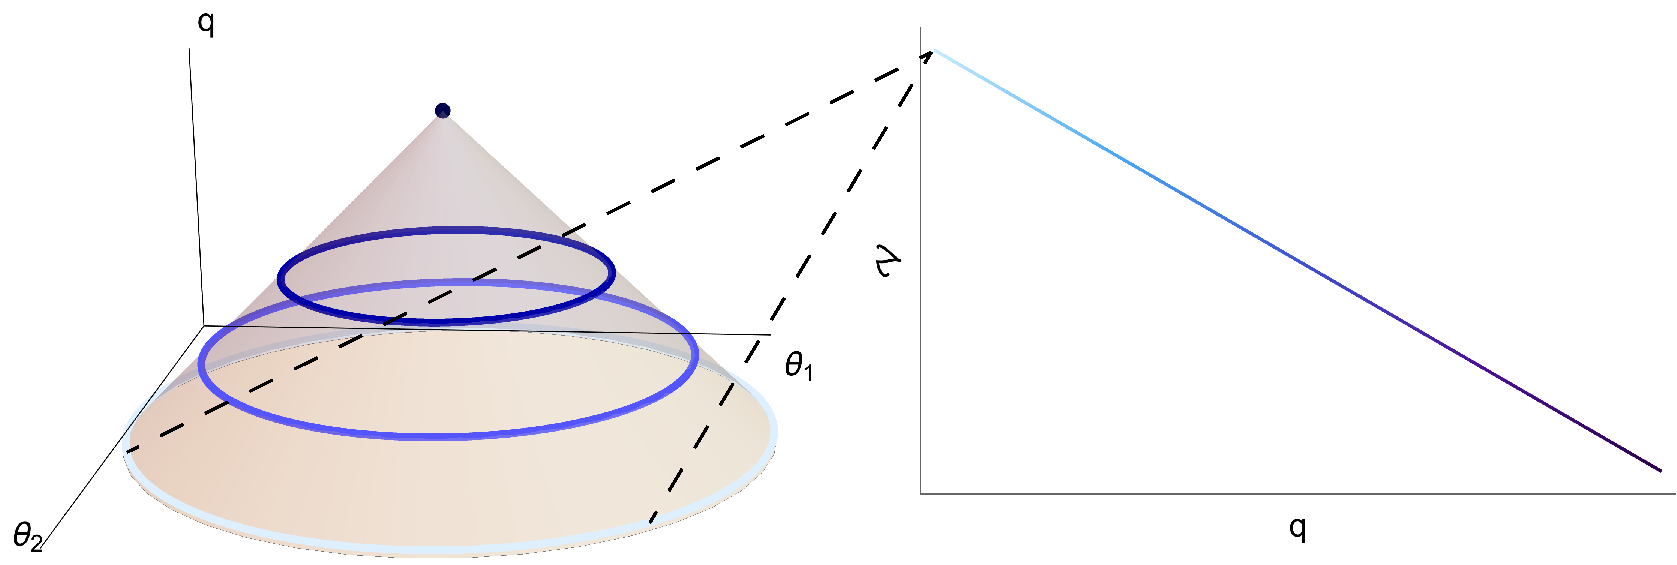
\includegraphics[width=\textwidth]{../figures/contour_volumes_redux.pdf}}
	\caption{\textbf{Left: An example output function $q(\theta_1,\theta_2)$ along with iso-output contours indicated (coloured lines). Right: The ``volume'' of output contours as a function of output value.} Note that here, since parameter space is two dimensional, the ``volume'' of each output value corresponds to a length of an iso-output contour.}
	\label{fig:contour_volumes}
\end{figure}

Solving our inverse problem requires determining the posterior distribution of parameter values, $p(\boldsymbol{\theta}|\hat{\Phi})$, which, when used as input to the forward map, results in the target distribution, $p(\boldsymbol{q}|\hat{\Phi})$. To derive the posterior parameter distribution, we consider the joint density of parameters and QOIs, $p(\boldsymbol{\theta},\boldsymbol{q}|\hat{\Phi})$. This can be decomposed in two ways using the law of conditional probability,
%
\begin{equation}\label{eq:joint}
  p( \boldsymbol{\theta}, \boldsymbol{q}|\hat{\Phi})
= p( \boldsymbol{\theta}|\boldsymbol{q}, \hat{\Phi}) \times p(\boldsymbol{q}|\hat{\Phi})
= p( \boldsymbol{q}|\boldsymbol{\theta}, \hat{\Phi}) \times p(\boldsymbol{\theta}|\hat{\Phi}).
\end{equation}
%
Rearranging eq. (\ref{eq:joint}), we obtain the posterior parameter distribution,
%
\begin{equation}\label{eq:posterior_mid}
p(\boldsymbol{\theta}|\hat{\Phi})
= \frac{p(\boldsymbol{\theta}|\boldsymbol{q}, \hat{\Phi}) \times p(\boldsymbol{q}|\hat{\Phi})}{p(\boldsymbol{q}| \boldsymbol{\theta}, \hat{\Phi})}.
\end{equation}
%
For a deterministic map, eq. \eqref{eq:posterior_mid} is only well defined when $\boldsymbol{q}=\boldsymbol{q}(\boldsymbol{\theta})$. (Since the mapping from parameters to outputs is deterministic, $p(\boldsymbol{q}| \boldsymbol{\theta}, \hat{\Phi})=\delta(\boldsymbol{q}(\boldsymbol{\theta}))$, i.e., the Dirac delta function centred at $\boldsymbol{q}=\boldsymbol{q}(\boldsymbol{\theta})$.)
 Thus eq. \eqref{eq:posterior_mid} becomes,
%
\begin{equation}\label{eq:posterior_mid1}
p(\boldsymbol{\theta}|\hat{\Phi})
= p(\boldsymbol{\theta}|\boldsymbol{q}(\boldsymbol{\theta}), \hat{\Phi}) \times p(\boldsymbol{q}(\boldsymbol{\theta})|\hat{\Phi}).
\end{equation}
%
In the same way that a single output value can be caused by any member of a set of parameter values, a target output distribution $p(\boldsymbol{q}|\hat{\Phi})$ can be caused by any member of a set of parameter distributions. To ensure uniqueness of the ``posterior'' parameter distributions, we must, therefore, specify ``prior'' distributions for the parameters, as in more traditional Bayesian inference. In what follows, we assume the conditional distribution $p(\boldsymbol{\theta}|\boldsymbol{q}, \hat{\Phi})$ is independent of the data, i.e., $p(\boldsymbol{\theta}|\boldsymbol{q}, \hat{\Phi})=p(\boldsymbol{\theta}|\boldsymbol{q})$, and thus represents a conditional ``prior'' which can be manipulated using Bayes' rule as,
%
\begin{equation}\label{eq:prior}
p(\boldsymbol{\theta}|\boldsymbol{q}(\boldsymbol{\theta})) = \frac{p(\boldsymbol{\theta})}{p(\boldsymbol{q}(\boldsymbol{\theta}))}.
\end{equation}
%
This results in the form of the posterior parameter distribution targeted by our sampling algorithm,
%
\begin{equation}\label{eq:posterior_input}
p(\boldsymbol{\theta}|\hat{\Phi}) = \frac{p(\boldsymbol{\theta})}{p(\boldsymbol{q}(\boldsymbol{\theta}))} p(\boldsymbol{q}(\boldsymbol{\theta})|\hat{\Phi}).
\end{equation}
%
Again, we defer to our companion piece \cite{lambert2018inverse} for detailed explanation of eqs. (\ref{eq:prior}) and (\ref{eq:posterior_input}) and, instead, here provide brief interpretation when considering a uniform prior on parameter space. In this case, $p(\boldsymbol{\theta}) = \frac{1}{V}$, where $V$ is the total volume of parameter space. The denominator term of eq. (\ref{eq:prior}) is the prior induced on output space by the prior over parameter space. For a uniform prior on parameter values, this is,
%
\begin{equation}\label{eq:contour_volume}
p(\boldsymbol{\theta}|\boldsymbol{q}(\boldsymbol{\theta})) = \frac{1}{\mathcal{V}(\boldsymbol{q}(\boldsymbol{\theta}))},
\end{equation}
%
where $\mathcal{V}(\boldsymbol{q}(\boldsymbol{\theta}))$ is the volume of parameter space occupied by the iso-output contour $\Omega(\boldsymbol{q}(\boldsymbol{\theta}))$ (see Fig. \ref{fig:contour_volumes} for the meaning of this volume for a two parameter example). Therefore, a uniform prior over parameter space implies a prior structure where all parameter values producing the same output are given equal weighting.

\subsection{Implementation of CMC}

Except for some toy examples, the denominator of eq. (\ref{eq:prior}) cannot be calculated, so exact sampling from the posterior parameter distribution of eq. (\ref{eq:posterior_input}) is not, in general, possible. We propose, instead, a computationally efficient sampling method to estimate $p(\boldsymbol{q}(\boldsymbol{\theta}))$, which forms the first step of our so-called ``Contour Monte Carlo'' (CMC) algorithm (Algorithm \ref{alg:cmc}; Figure \ref{fig:workflow}(ii)), where the volume of iso-output contours with each feasible output value is estimated. This step involves repeated independent sampling from the prior distribution of parameters, $\boldsymbol{\theta}^{[i]}\sim p(\boldsymbol{\theta}|\Xi)$, where $\Xi$ parameterises the prior probability density.
Each parameter sample is then mapped to an output value, $\boldsymbol{q}^{[i]}=\boldsymbol{q}(\boldsymbol{\theta}^{[i]})$. The collection of output samples is then fitted using a vine copula kernel density estimator (KDE) \cite{nagler2016evading}, $\hat{\Psi} = \argmax_\Psi p\left(\left( \boldsymbol{q}^{[1]}, \dots ,\boldsymbol{q}^{[N_1]} \right)|\Psi\right)$. Throughout the course of development of CMC, we tested many KDE methods and found vine copula KDE best suited to approximating the higher dimensional probability distributions required in practice -- other methods produced coarse estimates of the joint density and took substantially more computational resource. Indeed, the ability to do KDE in high dimensions was the motivation behind the creation of vine copula KDE in the first place \cite{nagler2016evading}. 


The second step in our algorithm then uses MCMC to sample from an approximate version of eq. (\ref{eq:posterior_input}), where the estimated density, $p(\boldsymbol{q}(\boldsymbol{\theta})|\hat{\Psi})$ replaces its corresponding estimand (Algorithm \ref{alg:cmc}; Figure \ref{fig:workflow}(iii)),
%
\begin{equation}\label{eq:posterior_input_estimated}
p(\boldsymbol{\theta}|\hat{\Phi},\Xi,\hat{\Psi}) =
\frac{p(\boldsymbol{\theta}|\Xi)}{p(\boldsymbol{q}(\boldsymbol{\theta})|\hat{\Psi})} \,
p(\boldsymbol{q}(\boldsymbol{\theta})|\hat{\Phi}).
\end{equation}
%
The final step in CMC is to compare output samples generated by MCMC with the target distribution (Figure \ref{fig:workflow}(iv)). As the sample size of both sampling steps (i.e. the contour volume estimation and MCMC steps) tends to infinity, CMC produces a sample of parameter values $(\boldsymbol{\theta}^{[1]},\boldsymbol{\theta}^{[2]},...)$ which, when mapped to the output space, corresponds to the target distribution $p(\boldsymbol{q}|\hat{\Psi})$. In developing CMC, we found that a finite sample of modest size for both steps of CMC results in parameter samples that, when transformed, often represented good approximations of the target. There are, however, occasions when this is not the case, and this final confirmatory step is indispensable since it frequently highlights inadequacies in contour volume estimation or MCMC, meaning more samples from either or both of these steps are required. It may also be necessary to tweak hyperparameters of the KDE in the contour volume estimation step to ensure reasonable approximation of the distribution of output values obtained by sampling the prior density.

If the target distribution is sensitive to the contour volume estimates, this may also indicate that the target snapshot distribution is incompatible with the model: here, we make no claims on existence of a solution to the inverse problem, only that, Contour Monte Carlo is a pragmatic approach to approximate it by sampling if one should exist. A useful way to diagnose whether the target distribution can be produced from the model and chosen priors is to plot the output values from the contour volume estimation step of CMC: this is akin to visualising the prior predictive distribution in traditional Bayesian inference \cite{lambert2018Student}. If the bulk of target probability mass does not overlap with the simulated output values, then the model and/or chosen prior are unlikely to be invertible to this particular target. In \S\ref{sec:4D} and \S\ref{sec:hesc}, we provide examples that illustrate this aspect of model checking.

\subsection{Workflow and CMC algorithm}

A graphical illustration of the complete CMC workflow is provided in Figure \ref{fig:workflow}. All variables are defined in Table \ref{tab:variable_glossary}. The CMC algorithm is provided in Algorithm \ref{alg:cmc}. In this implementation, MCMC sampling is performed via the Random Walk Metropolis algorithm, but for the examples in \S \ref{sec:results}, we use an adaptive MCMC algorithm to improve sampling efficiency \cite{johnstone2016uncertainty}.

\begin{figure}[H]
  \centerline{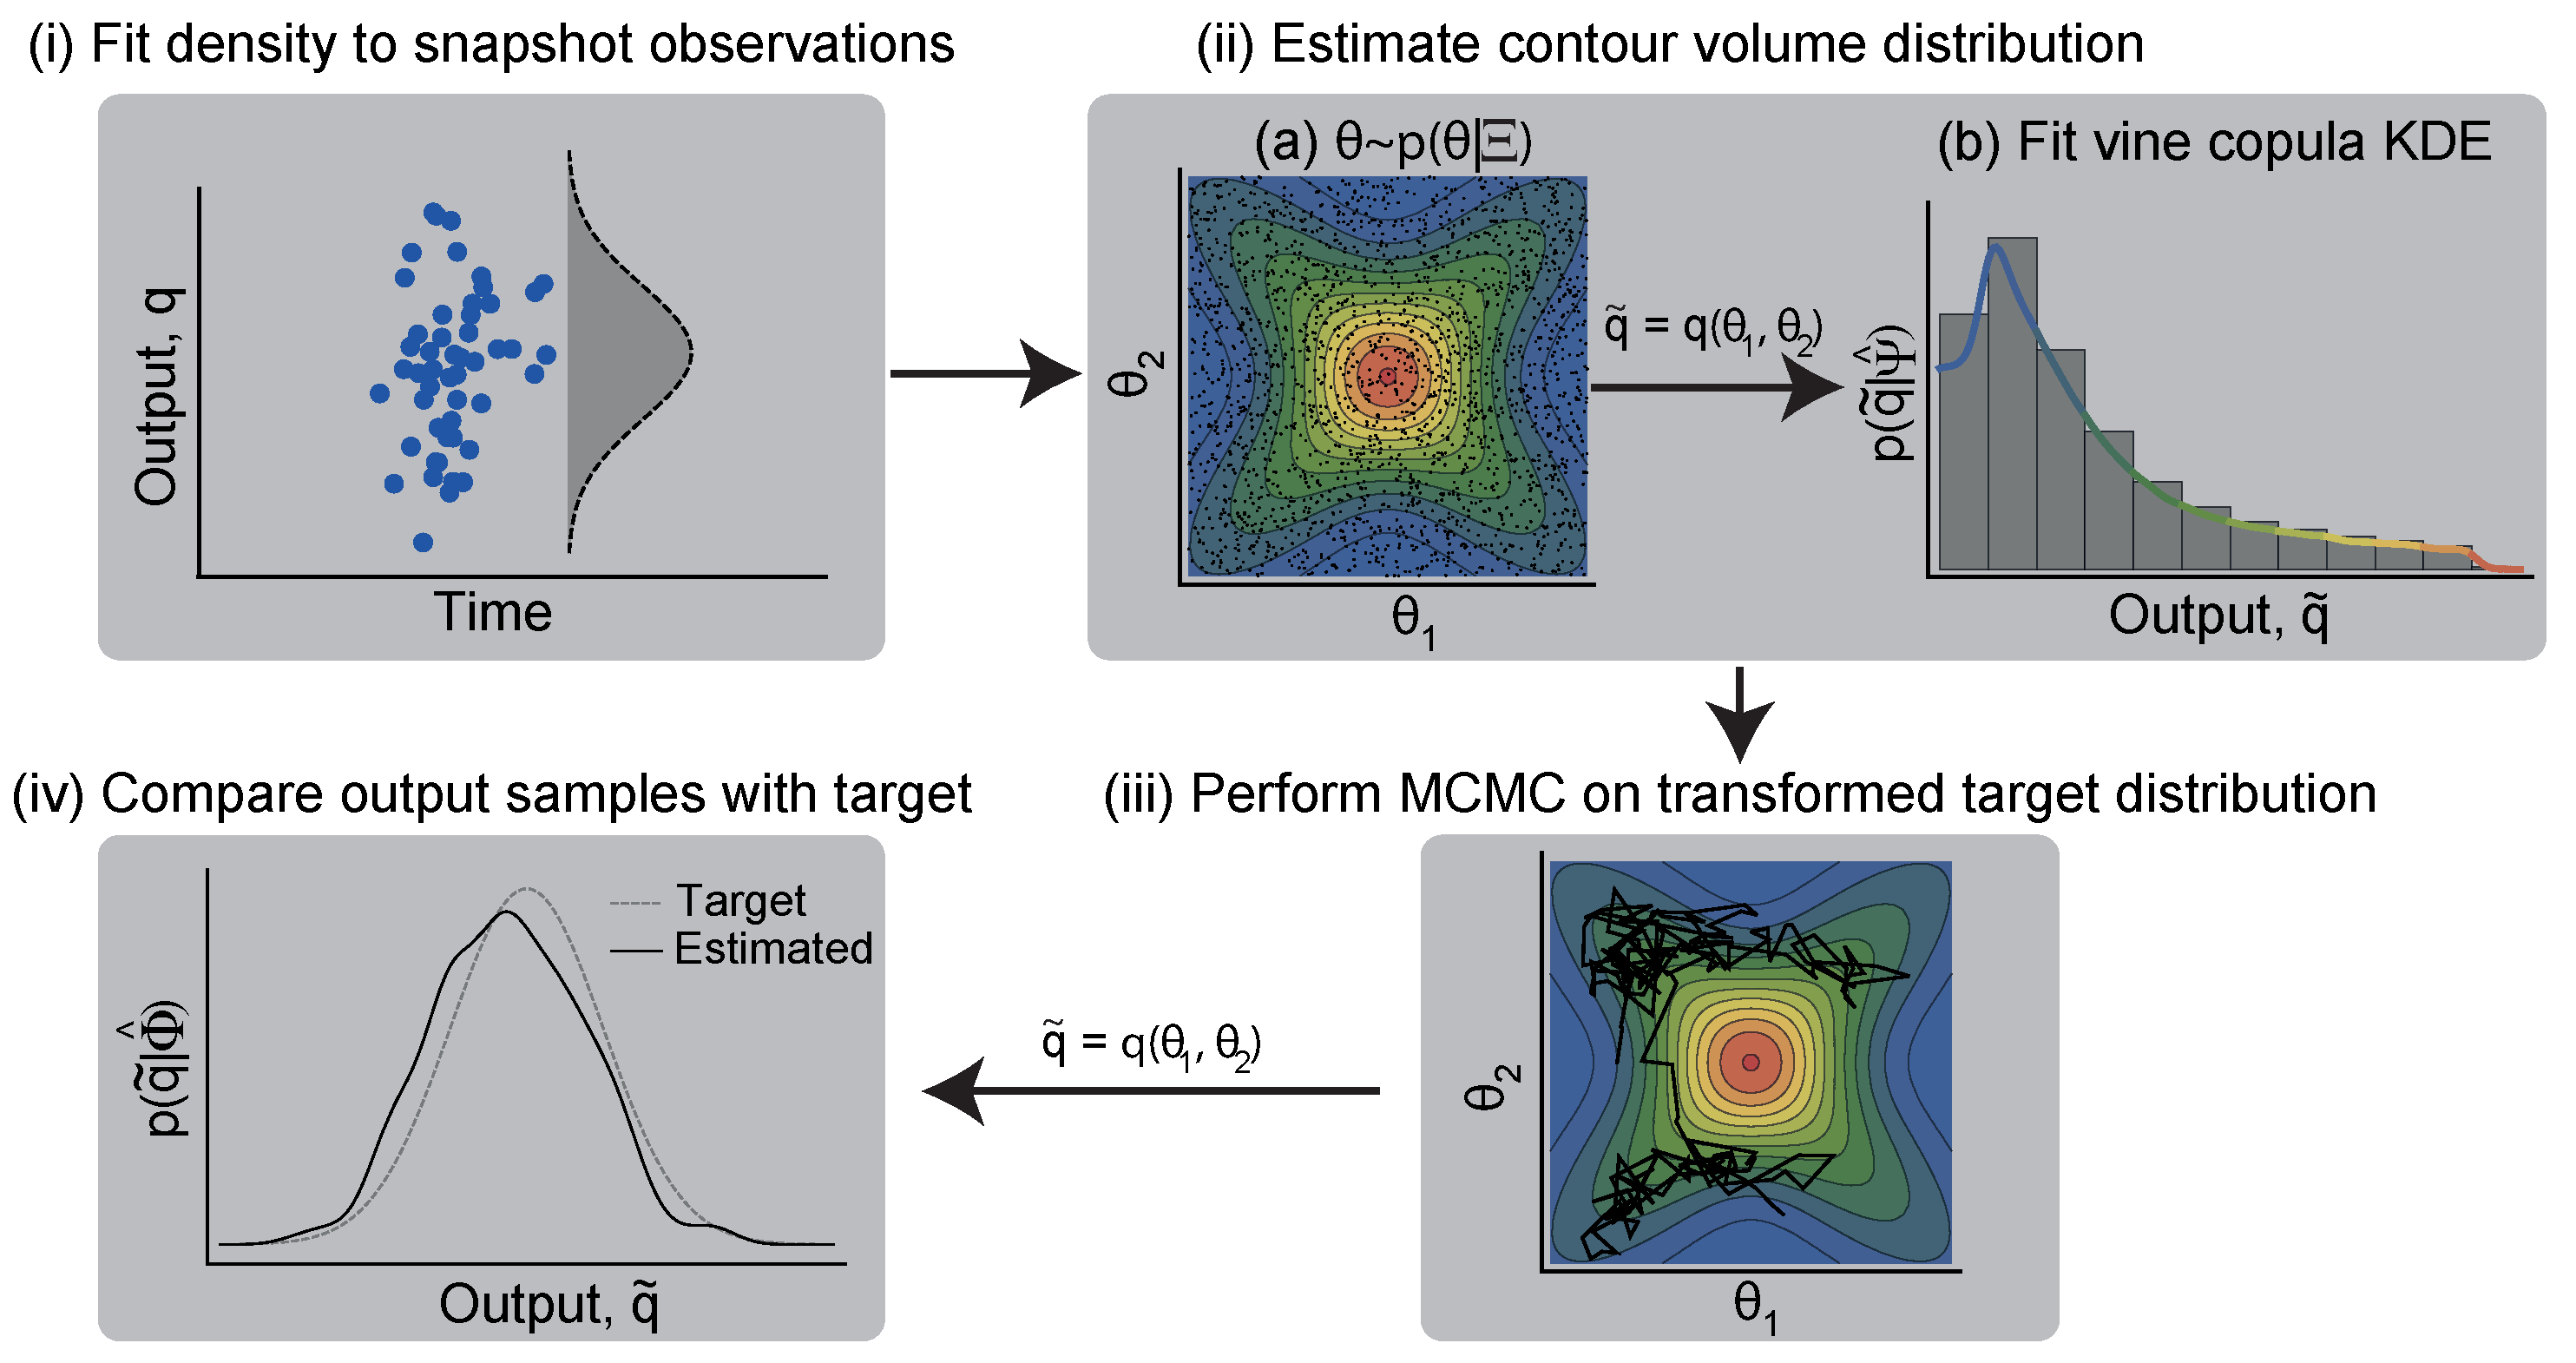
\includegraphics[width=1.0\textwidth]{../figures/workflow.pdf}}
  \caption{\textbf{Workflow for Contour Monte Carlo to estimate cell population heterogeneity.} The distribution targeted in (iii) is given by eq. (\ref{eq:posterior_input_estimated}). Here, $\tilde q$ is used to represent an output value resultant from applying the functional $q$ to parameter samples $(\theta_1,\theta_2)$.}
  \label{fig:workflow}
\end{figure}

\begin{algorithm}[H]
\footnotesize
\texttt{\\}
\begin{algorithmic}
\Procedure{CMC}{$\boldsymbol{Y}, \Xi, N_1, N_2$}\Comment{Sample from posterior parameter distribution}
	\State $\hat{\Phi} = \Call{SnapshotEstimator}{\boldsymbol{Y}}$
	\State $\hat{\Psi} = \Call{ContourVolumeEstimator}{\Xi,N_1}$
	\State $\left(\boldsymbol{\theta}^{[1]},...,\boldsymbol{\theta}^{[N_2]}\right) = \Call{MCMC}{\hat{\Phi},\Xi, \hat{\Psi},N_2}$
	\State $\text{converged} = \Call{CompareOutputToTarget}{(\boldsymbol{\theta}^{[1]},...,\boldsymbol{\theta}^{[N_2]}), \hat{\Phi}}$
	\While{converged$\neq$1} \Comment{Rerun contour volume estimation (if necessary modify vine copula KDE hyperparmeters) and/or MCMC, with larger sample sizes if required}
		 \State $\hat{\Psi}=\Call{ContourVolumeEstimator}{\Xi, N_1'},\; N_1' \geq N_1$
         \State $\left( \boldsymbol{\theta}^{[1]},...,\boldsymbol{\theta}^{[N_2']} \right)
                = \Call{MCMC}{\hat{\Phi},\Xi, \hat{\Psi},N_2'}, \; N_2' \geq N_2$
          \State $\text{converged} = \Call{CompareOutputToTarget}{(\boldsymbol{\theta}^{[1]},...,\boldsymbol{\theta}^{[N_2']} ), \hat{\Phi}}$
          \State $N_1 \leftarrow N_1', \; N_2 \leftarrow N_2'$
	\EndWhile
	\State \Return $\left( \boldsymbol{\theta}^{[1]},...,\boldsymbol{\theta}^{[N_2]} \right)$
\EndProcedure
\end{algorithmic}

\texttt{\\}
\begin{algorithmic}
\Procedure{SnapshotEstimator}{$\boldsymbol{Y}$}\Comment{Fit snapshots with kernel density estimator (KDE)}
	\State $\hat{\Phi} = \argmax_\Phi p(\boldsymbol{Y}|\Phi)$
	\State \Return $\hat{\Phi}$
\EndProcedure
\end{algorithmic}
	
\texttt{\\}
\begin{algorithmic}
\Procedure{ContourVolumeEstimator}{$\Xi, N_1$}\Comment{Estimate volume of contours}
	\For{$i$ in $1:N_1$}
		\State $\boldsymbol{\theta}^{[i]} \sim p(\boldsymbol{\theta}|\Xi)$           \Comment{Sample from prior density}
		\State $\boldsymbol{q}^{[i]} = \boldsymbol{q}(\boldsymbol{\theta}^{[i]})$  \Comment{Calculate corresponding output value}
	\EndFor
	\State $ \hat{\Psi} = \argmax_\Psi p\left(\left( \boldsymbol{q}^{[1]}, \dots ,\boldsymbol{q}^{[N_1]} \right)|\Psi\right)$
           \Comment{Fit vine copula KDE}
	\State \Return $\hat{\Psi}$
\EndProcedure
\end{algorithmic}

\texttt{\\}
\begin{algorithmic}
\Procedure{MCMC}{$\hat{\Phi},\Xi, \hat{\Psi}, N_2$}\Comment{Random Walk Metropolis algorithm targeting posterior parameter distribution}
	\State $\boldsymbol{\theta}^{[0]} \sim \pi(.)$ \Comment{Sample from arbitrary initialisation distribution}
	\For{$i$ in $1:N_2$}
		\State $\boldsymbol{\theta}^{[i]^\prime}\sim \mathcal{N}(\boldsymbol{\theta}^{[i-1]},\boldsymbol{\Sigma})$ \Comment{Propose new parameter values}
		\State
		\Comment{Calculate Metropolis acceptance ratio}
		\State $r =
                     p(\boldsymbol{\theta}^{[i]^\prime}|\Xi) \
                     p(\boldsymbol{q}(\boldsymbol{\theta}^{[i-1]})|\hat{\Psi}) \
                     p(\boldsymbol{q}(\boldsymbol{\theta}^{[i]^\prime})|\hat{\Phi})
                     /
                     \left[
                     p(\boldsymbol{\theta}^{[i-1]}|\Xi) \
                     p(\boldsymbol{q}(\boldsymbol{\theta}^{[i]^\prime})|\hat{\Psi}) \
                     p(\boldsymbol{q}(\boldsymbol{\theta}^{[i-1]})|\hat{\Phi})
                     \right]$
		\State $u\sim U(0,1)$ \Comment{Sample from uniform distribution}
		\If{$r > u$}
		    \State $\boldsymbol{\theta}^{[i]} = \boldsymbol{\theta}^{[i]^\prime}$ \Comment{Accept proposal}
		\Else
		    \State $\boldsymbol{\theta}^{[i]} = \boldsymbol{\theta}^{[i-1]}$ \Comment{Reject proposal}
		\EndIf
	\EndFor
	\State \Return $\left( \boldsymbol{\theta}^{[1]},...,\boldsymbol{\theta}^{[N_2]} \right)$
\EndProcedure
\end{algorithmic}

\texttt{\\}
\begin{algorithmic}
\Procedure{CompareOutputToTarget}{$(\boldsymbol{\theta}^{[1]},...,\boldsymbol{\theta}^{[N_2]}), \hat{\Phi}$}\Comment{Check output distribution close to target}
	\For{$i$ in $1:N_2$}
		\State $\tilde{\boldsymbol{q}}^{[i]} = \boldsymbol{q}(\boldsymbol{\theta}^{[i]})$ \Comment{Compute QOIs for each parameter sample}
	\EndFor
	\If{$ p(\tilde{\boldsymbol{q}}) \approx p(\tilde{\boldsymbol{q}}|\hat{\Phi})?$} \Comment{Compare sampled output distribution with target}
		\State \Return 1 \Comment{If sufficiently close then converged}
	\Else
		\State \Return 0
	\EndIf
\EndProcedure
\end{algorithmic}

\caption{Pseudocode for the Contour Monte Carlo algorithm for sampling from the posterior parameter distribution of eq. (\ref{eq:posterior_input_estimated}). }\label{alg:cmc}
\end{algorithm}

To generate our results in \S\ref{sec:results}, we assumed for the contour volume estimation step sample sizes were sufficient if the output samples from MCMC provided a reasonable approximation to the target, although we recognise that future work should refine this process further. For the MCMC step, we used adaptive covariance MCMC (see SOM of \cite{johnstone2016uncertainty}) to sample from the target distribution, as it typically provides a considerable speed-up over Random Walk Metropolis \cite{metropolis1953equation,lambert2018Student}. We also used the Gelman-Rubin convergence statistic, $\hat{R}$, to diagnose convergence \cite{lambert2018Student,gelman1992inference}, with a convergence threshold of $\hat{R}\leq\sim 1.1$.

To solve the forward model of each differential equation, we used Julia's \cite{bezanson2017julia} ``solve'' method for ODE models from the ``DifferentialEquations.jl'' library \cite{rackauckas2017differentialequations}, which automatically chooses an efficient inbuilt solver. To replicate the results in this section, we recommend readers execute the corresponding Julia scripts (one for each result section) at \url{https://github.com/ben18785/inverse-sensitivity/tree/master/examples}. Note that, these scripts use the ``\textit{RCall}'' library for Julia \cite{batesRCall}, which calls \textsf{R} from Julia. This package was necessary to use the ``\textit{kdevine}'' \textsf{R} package for vine copula kernel density estimation \cite{naglerkdevine2018}.

\section{Results}\label{sec:results}
In this section, we use CMC to estimate the posterior parameter distribution for three biological systems.
% of interest targeting synthetic parametric densities. That is,
In all but one of the examples, we assume that the first step of CMC (``SnapshotEstimator'' within Algorithm \ref{alg:cmc}) has already been undertaken and we are faced with inferring a parameter distribution which, when mapped to outputs, recapitulates the target density. To accompany the text, we provide the Julia notebook used to generate the results. %, which we hope will be of use to others wanting to apply CMC to estimate cell population heterogeneity.
A table of priors used for each example is provided in Table \ref{tab:priors}.


\subsection{Growth factor model}
We first consider the ``growth factor model'' introduced by \cite{dixit2018maximum}, which concerns the dynamics of inactive ligand-free cell surface receptors $R$ and active ligand-bound cell surface receptors $P$, modulated by an exogenous ligand $L$. The governing dynamics are determined by the following system,
%
\begin{align}\label{eq:growth_factor}
\frac{dR}{dt} &= R_T k_{deg} + k_1 L R(t) + k_{-1} P(t) - k_{deg} R(t)\\
\label{eq:growth_factor1}
\frac{dP}{dt} &= k_1 L R(t) - k_{-1} P(t) - k^*_{deg} P(t),
\end{align}
with initial conditions,
\begin{equation*}
R(0) = 0.0, \qquad P(0) = 0.0,
\end{equation*}
%
where $\boldsymbol{\theta}=(R_T, k_1, k_{-1}, k_{deg}, k^*_{deg})$ are parameters to be determined. In this example, we use measurements of the active ligand-bound receptors $P$ to estimate cellular heterogeneity in processes. We denote the solution of eq. (\ref{eq:growth_factor1}) as $P(t; \boldsymbol{\theta}, L)$ and seek to determine the parameter distribution consistent with an output distribution,
%
\begin{equation}\label{eq:MM_outputDistribution}
\boldsymbol{q} =
\begin{pmatrix}
q_1\\
q_2\\
\end{pmatrix}
=
\begin{pmatrix}
P(10; \boldsymbol{\theta}, 2)\\
P(10; \boldsymbol{\theta}, 10)\\
\end{pmatrix} \sim  \mathcal{N}
\begin{bmatrix}
\begin{pmatrix}
2\times 10^4\\
3\times 10^4\\
\end{pmatrix}, \;\;
\begin{pmatrix}
1\times 10^5 & 0\\
0 & 1\times 10^5\\
\end{pmatrix}
\end{bmatrix}.
\end{equation}
%

\subsubsection{Uniform prior}
To start, we specify a uniform prior for each of the five parameters, with bounds given in Table \ref{tab:priors}. To estimate the posterior parameter distribution, we use CMC, with adaptive covariance MCMC \cite{johnstone2016uncertainty} for the second step.

In Figure \ref{fig:growth_factor_outputs}A, we show the sampled outputs (blue points) versus the contours of the target distribution (black solid closed curves), illustrating a good correspondence between the sampled and target densities. Above and to the right of the main panel, we also display the marginal target densities (solid black lines) versus kernel density estimator reconstructions of the output marginals from the CMC samples (dashed blue lines), which again highlights the fidelity of the CMC sampled density to the target.

\begin{figure}[H]
	\centerline{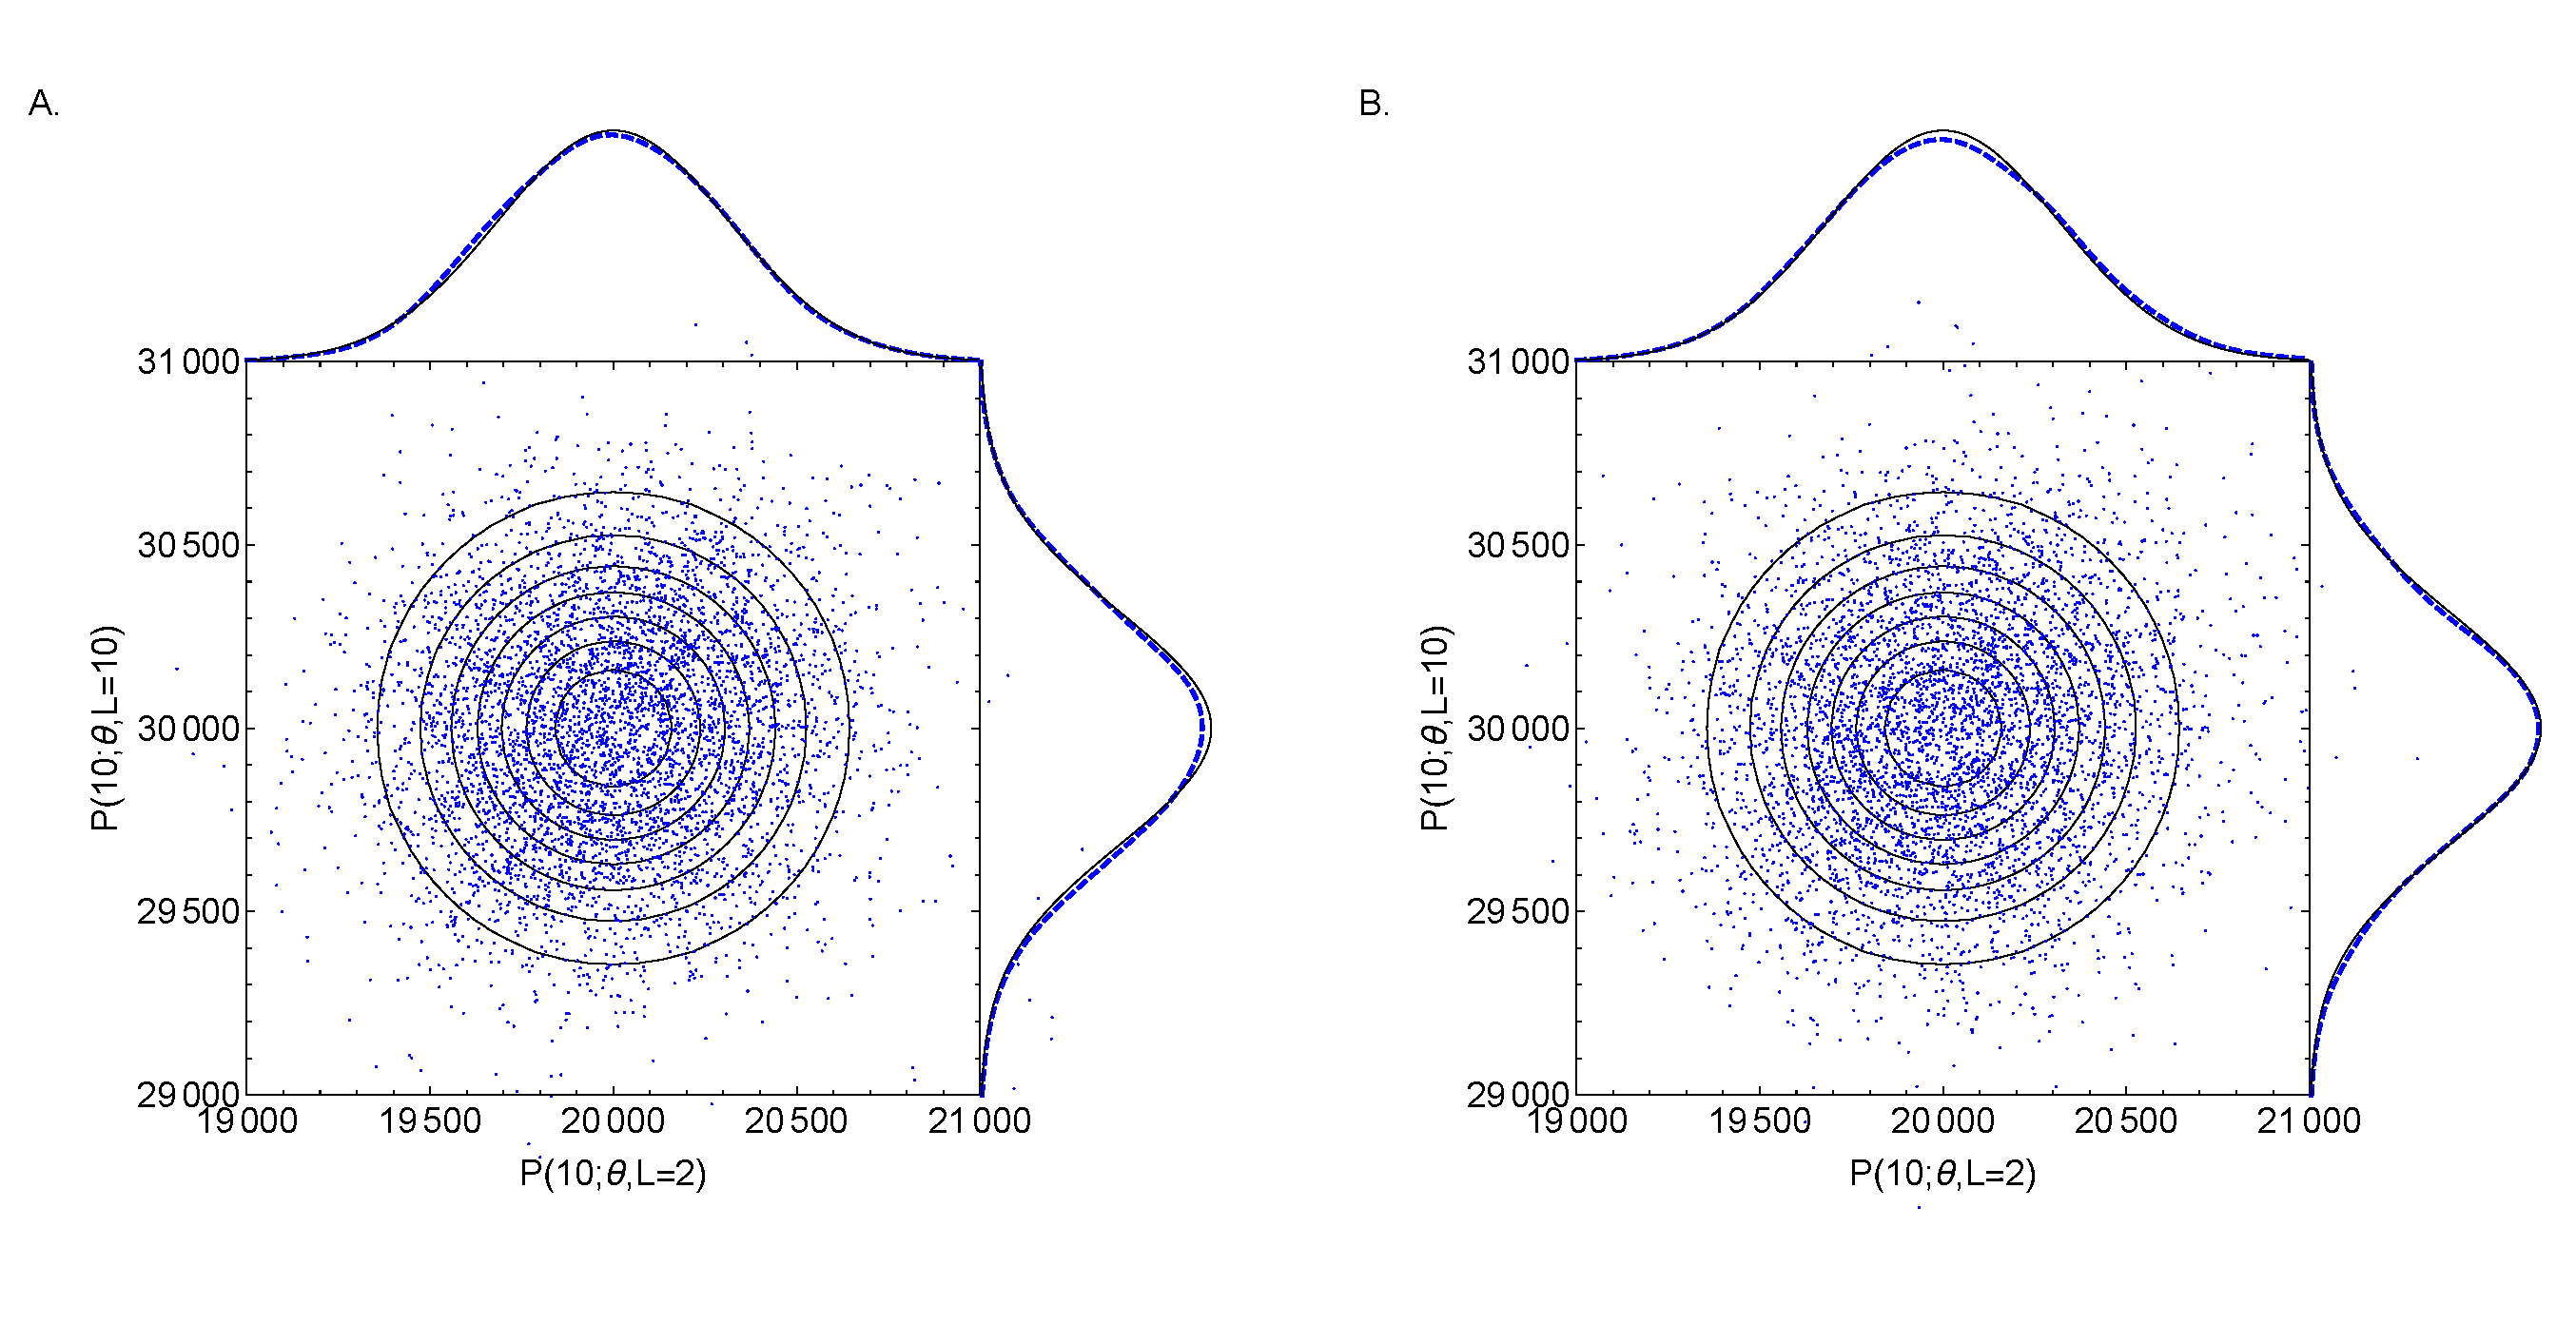
\includegraphics[width=\textwidth]{../figures/growth_factor_outputs.pdf}}
	\caption{\textbf{The target joint output distribution (solid contour lines) and target marginal distributions (solid lines; above and to side of figure) versus outputs sampled by CMC (blue points) and reconstructed marginals (dashed lines) for (A) uniform and (B) normal parameter priors.} In CMC, 100,000 independent samples were used in the ``ContourVolumeEstimator'' step and 10,000 MCMC samples across each of 4 Markov chains were used in the second step, with the first half of the chains discarded as ``warm-up'' \cite{lambert2018Student}. For the reconstructed marginal densities in the plots, we use Mathematica's ``SmoothKernelDistribution'' function specifying bandwidths of 100 with Gaussian kernels \cite{mathematica}.}
	\label{fig:growth_factor_outputs}
\end{figure}

In Figure \ref{fig:growth_factor_inputs}A, we plot the joint posterior parameter distribution for $k_1$, the rate of ligand binding to inactive receptors, and $k_{-1}$, which dictates the rate of the reverse reaction, where the ligands unbind. The output measurements we used to fit the model correspond to levels of the bound ligands, which can be generated whenever the ratio of $k_1$ to $k_{-1}$ is approximately given by the corresponding steady state ratio. Because of this, the distribution representing cell process heterogeneity contains linear positive correlations between these parameters. In Figure \ref{fig:growth_factor_inputs}B, we show the posterior parameter distribution for $k_{deg}$, the rate of degradation of ligand-free cell surface receptors and $R_T$, which dictates the rate of introduction of ligand-free cell surface receptors, which shows a concentrated region of posterior probability mass. Why can we better resolve $(k_{deg},R_T)$ compared to $(k_1,k_{-1})$ from our measurements? To answer this, it is useful to calculate the sensitivity of $P(t; \boldsymbol{\theta}, L)$ to changes in each of the parameters. To account for the differing magnitudes of each parameter, we calculate elasticities, the proportional changes in measured output for a proportional change in parameter values, using the forward sensitivities method described in \cite{DGCT2018}, which are shown in Figure \ref{fig:dixit_elasticities}. When the exogenous ligand is set $L=2$, these indicate the active ligand-bound receptor concentration is most elastic to changes in $R_T$ and $k_{deg}$, meaning that their range is more restricted by the output measurement than for $k_1$ and $k_{-1}$, which have elasticities at $t=10$ closer to 0. In Table \ref{tab:growth_factor_results}, we show the posterior quantiles for the estimated parameters and, in the last column, indicate the ratio of the 25\%-75\% posterior interval widths to the uniform prior range for each parameter. These were strongly negatively correlated with the magnitude of the elasticities for each parameter ($\rho=0.95$, $t=-5.22$, $df=3$, $p=0.01$ Pearson's product-moment correlation), indicating the utility of sensitivity analyses for optimal experimental design. We would suggest however that CMC can also be used for this purpose, using synthetic data in place of real measurements.


\begin{figure}[H]
	\centerline{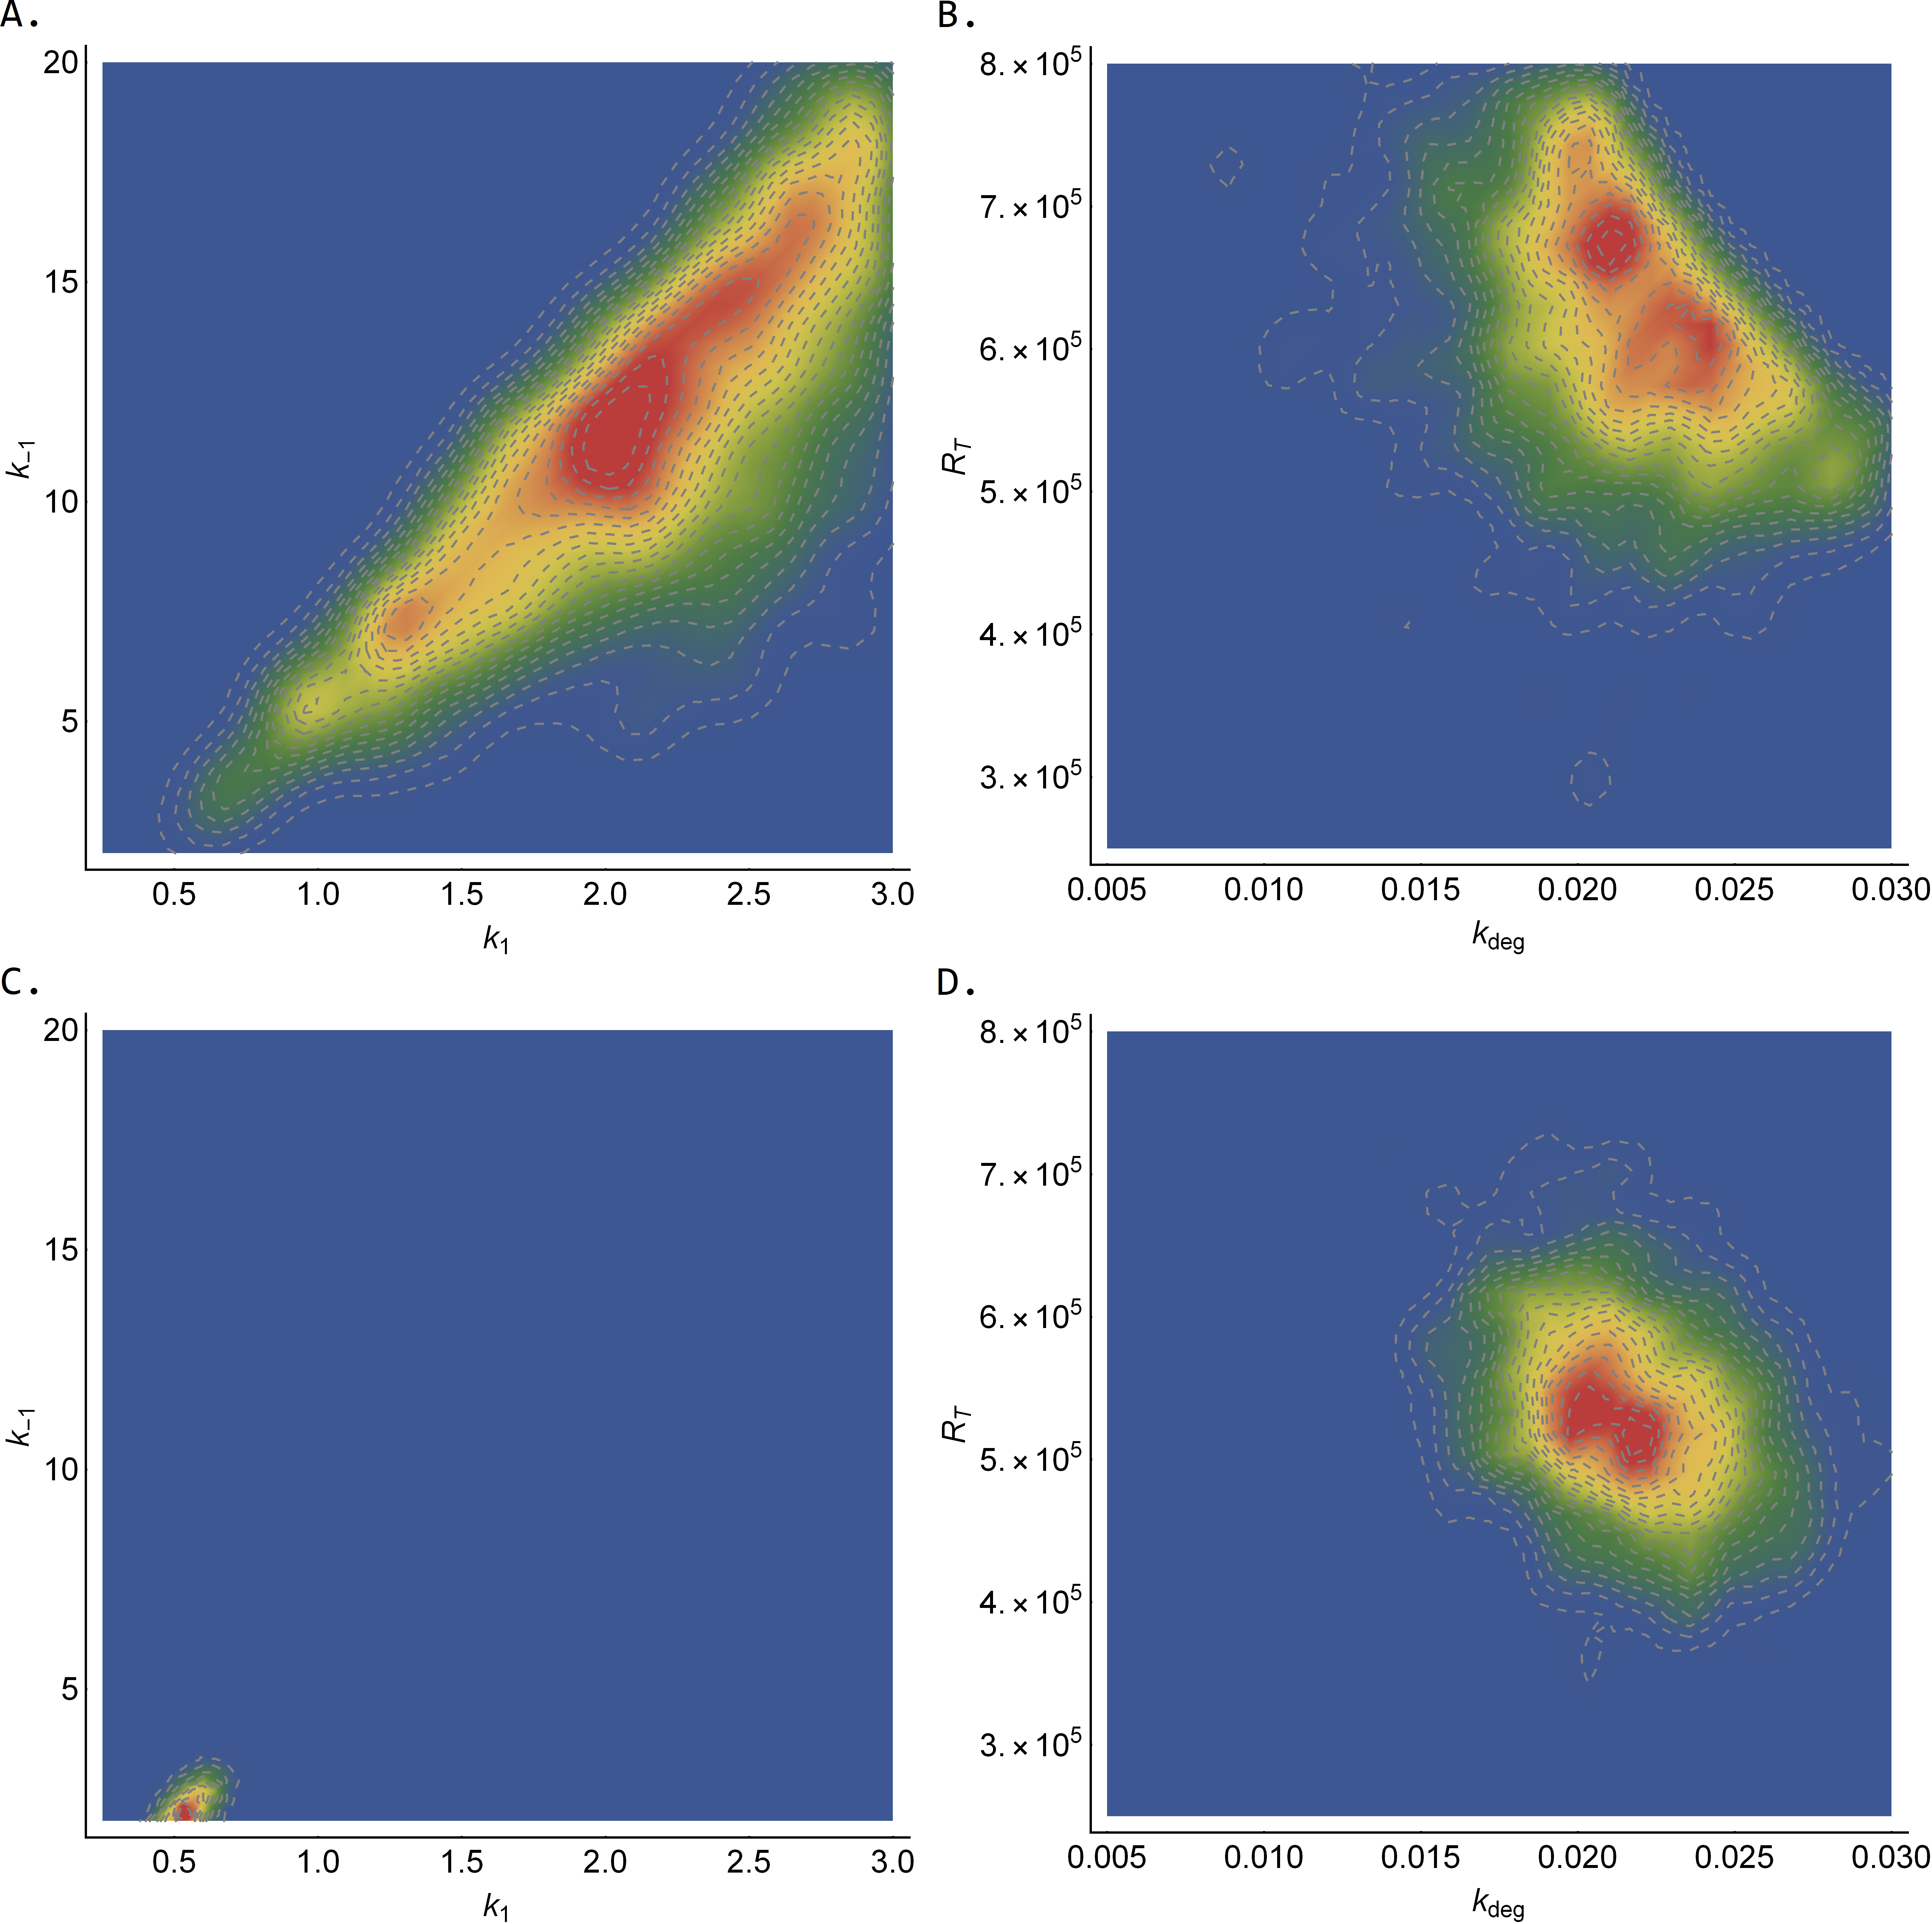
\includegraphics[width=\textwidth]{../figures/growth_factor_inputs.png}}
	\caption{\textbf{The joint posterior distributions of $(k_1,k_{-1})$ (left-column) and $(k_{deg},R_T)$ for the growth factor model estimated by CMC sampling using uniform priors (top row) and normal priors (bottom row).} See Figure \ref{fig:growth_factor_outputs} caption for CMC details and Table \ref{tab:priors} for the priors used. Red (blue) indicates areas of relatively high (low) probability mass.}
	\label{fig:growth_factor_inputs}
\end{figure}

\begin{figure}[H]
	\centerline{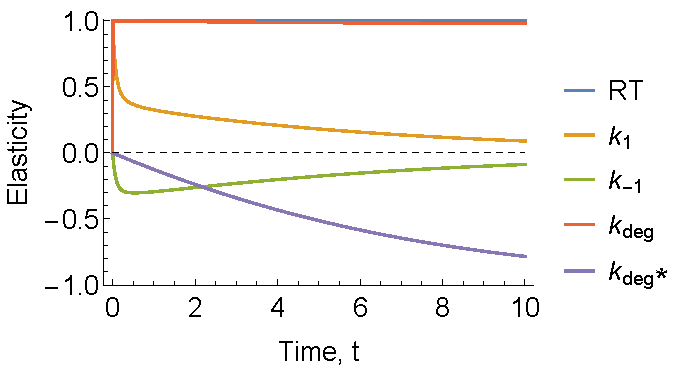
\includegraphics[width=0.7\textwidth]{../figures/dixit_elasticities.pdf}}
	\caption{\textbf{The elasticities of the measured concentration of active ligand-bound receptors $P$ versus time when $L=2$.} When calculating the elasticities of each parameter, the other parameters were set to their posterior medians given in Table \ref{tab:growth_factor_results}.}
	\label{fig:dixit_elasticities}
\end{figure}

\subsubsection{Normal prior}
For an unidentified model, there is typically a multitude of possible probability distributions over parameter values which map to the same target output distribution. To reduce the space of posterior parameter distributions to one, it is therefore necessary to specify a prior parameter distribution. It is also preferable to allow priors to influence estimates in studies of cellular heterogeneity, since this allows incorporation of pre-existing biological knowledge with compensatory reductions in estimator variance. CMC accommodates different prior choices, with both the ``ContourVolumeEstimation'' step and the acceptance ratio in the ``MCMC'' step (Algorithm \ref{alg:cmc}) being affected in such a way that posterior parameter distribution maps to the same output target. We now use CMC to estimate the posterior parameter distribution when changing from uniform priors to more concentrated normal priors (prior hyperparameters shown in Table \ref{tab:priors}). As desired, the target output distribution appears invariant (Figure \ref{fig:growth_factor_outputs}B) although with substantial changes in the posterior parameter distributions (Figure \ref{fig:growth_factor_inputs}C\&D). In particular, the posterior distributions obtained from shifting to the normal prior are more concentrated in parameter space compared to the uniform case (rightmost column of Table \ref{tab:growth_factor_results}). The differences in posterior distribution resultant from changes to priors are likely to be more marked the less definitive a guide the data provides on the underlying process and, hence, can be used to stabilise the resultant inferences according to external knowledge about the system.

\begin{table}
%	\scriptsize
\begin{tabular}{c|ccccc|c}
\toprule
&&&&&&                                         Posterior \\
Parameter &  \multicolumn{5}{c}{Quantiles} &   25\%-75\% \\
          & 2.5\% & 25\% & 50\% & 75\% & 97.5\% & conc.\\
\toprule
\multicolumn{7}{c}{Uniform prior} \\
\toprule
$R_T$       &  441,006 & 548,275 & 606,439 & 677,055 & 772,484 & 23\%\\
$k_1$       &  0.90 & 1.69 & 2.17 & 2.56 & 2.95 & 32\%\\
$k_{-1}$    & 4.35 & 8.35 & 11.23 & 14.23 & 18.71 & 33\%\\
$k_{deg}$   & 0.013 & 0.019 & 0.021 & 0.024 & 0.029 & 20\%\\
$k^*_{deg}$ & 0.20 & 0.34 & 0.40 & 0.44 & 0.49 & 27\%\\
\toprule
\multicolumn{7}{c}{Normal prior} \\
\toprule
$R_T$       & 408,396 & 487,372 & 529,558 & 577,970 & 678,632 & 16\%\\
$k_1$       & 0.39 & 0.49 & 0.54 & 0.60 & 0.70 & 4\%\\
$k_{-1}$    & 1.39 & 1.92 & 2.26 & 2.63 & 3.35 & 4\%\\
$k_{deg}$   & 0.016 & 0.020 & 0.022 & 0.024 & 0.027 & 16\%\\
$k^*_{deg}$ & 0.22 & 0.29 & 0.33 & 0.38 & 0.46 & 21\%\\
\end{tabular}
\caption{\textbf{Estimated quantiles from CMC samples for the growth factor model with uniform and normal priors.} The last column indicates the proportion of the uniform prior bounds occupied by the 25\%-75\% posterior interval in each case. The particular priors used in each case are given in Table \ref{tab:priors}.}
\label{tab:growth_factor_results}
\end{table}

\subsection{Michaelis-Menten kinetics}
In this section, we use CMC to invert output measurements from the Michaelis-Menten model of enzyme kinetics (see, for example, \cite{murray2007mathematical}); illustrating the capability of CMC to resolve population substructure from multimodality of the output distribution. The Michaelis-Menten model of enzyme kinetics describes the dynamics of concentrations of an enzyme ($E$), a substrate ($S$), an enzyme-substrate complex ($ES$), and a product ($P$). Specifically,
%
\begin{equation}\label{eq:michaelis_menten}
\begin{aligned}
\frac{dE}{dt} &= -k_f E(t)S(t) + k_r C(t) + k_{cat} C(t), \\
\frac{dS}{dt} &= -k_f E(t)S(t) + k_r C(t), \\
\frac{dC}{dt} &= \phantom{-}k_f E(t)S(t) - k_r C(t) - k_{cat} C(t), \\
\frac{dP}{dt} &= \phantom{-}k_{cat} C(t),
\end{aligned}
\end{equation}
%
with initial conditions,
\begin{equation}
E(0) = E_0, \; S(0)=S_0, \; C(0)=C_0, \; P(0)=P_0,
\end{equation}
%
where $k_f$ is the rate constant for the forward reaction $E+S \rightarrow C$, $k_r$ is the rate of the reverse reaction $C \rightarrow E+S$, and $k_{cat}$ is the catalytic rate at which the product is formed by the reaction $C \rightarrow E + P$.


\subsubsection{Bimodal output distribution}

When subpopulations of cells, each with distinct dynamics, are thought to exist, determining their characteristics - proportions of overall cell number, likely parameter values, and so on - is often of key interest \cite{hasenauer2011identification,loos2018hierarchical}. Before formal inference occurs, multi-modality of the output distribution may signal the existence of fragmented subpopulations of cells. Here we target the following bimodal bivariate normal distribution,
%
\begin{align}
\boldsymbol{q} = \begin{pmatrix} q_1 \\ q_2 \end{pmatrix}
 = \begin{pmatrix} E(2; \boldsymbol{\theta}) \\ S(1; \boldsymbol{\theta}) \end{pmatrix}
&  \sim
p(\boldsymbol{q}; \boldsymbol{\mu}_1,\Sigma_1, \boldsymbol{\mu}_2, \Sigma_2) \\
&= \frac{1}{2}\left(\mathcal{N}(\boldsymbol{q}; \boldsymbol{\mu}_1,\Sigma_1)
+ \mathcal{N}(\boldsymbol{q}; \boldsymbol{\mu}_2,\Sigma_2)\right),
\end{align}
%
%where $\boldsymbol{x} = \left(E(2; \boldsymbol{\theta}), S(1; \boldsymbol{\theta})\right)$ with each element corresponding to the solutions of eq. (\ref{eq:michaelis_menten}) for the enzyme and substrate at times $t=2$ and $t=1$, respectively, and
where $\boldsymbol{\theta}=(k_f,k_r,k_{cat})$. The parameters of the mixture normal output distribution we target are
\begin{equation*}
\begin{aligned}
&\boldsymbol{\mu}_1=[2.2, 1.6]', \; \Sigma_1 = \begin{pmatrix}0.018 & -0.013 \\ -0.013 & 0.010 \end{pmatrix}, \\
&\boldsymbol{\mu}_2=[2.8, 1.0]', \; \Sigma_2 = \begin{pmatrix}0.020 & -0.010 \\ -0.010 & 0.020 \end{pmatrix}.
\end{aligned}
\end{equation*}
In what follows, we specify uniform priors on each of the elements of $\boldsymbol{\theta}$ (see Table \ref{tab:priors}).


Using a modest number of samples in each step, CMC was able to recapitulate the output target distribution (Figure \ref{fig:mm_bimodal_inputs_outputs}A). Without specifying \textit{a priori} information on the subpopulations of cells, two distinct clusters of cells emerged from application of CMC (orange and blue points in Figure \ref{fig:mm_bimodal_inputs_outputs}B), each corresponding to distinct modes of the output distribution (corresponding coloured points in Figure \ref{fig:mm_bimodal_inputs_outputs}A). It is worth noting however that the issues inherent with MCMC sampling of multimodal distributions similarly apply here and so, whilst here adaptive MCMC \cite{johnstone2016uncertainty} sufficed to explore the posterior surface, it may be necessary to use MCMC methods known to be robust to such geometries (for example, population MCMC \cite{jasra2007population}).

\begin{figure}[H]
\centerline{\includegraphics[width=\textwidth]{../figures/mm_bimodal_inputs_outputs.pdf}}
\caption{\textbf{Michaelis-Menten model. (A) Bimodal target distribution $\boldsymbol{q}$ (solid contour lines) versus output samples (points). (B) Posterior parameter samples (points).} The solid and dashed lines above and to the side of panel A indicate the target and estimated marginal output distributions, respectively. The orange (blue) points in A were generated by the orange (blue) parameter samples in B. See Figure \ref{fig:growth_factor_outputs} caption for CMC details. Mathematica's ``SmoothKernelDistribution'' function \cite{mathematica} with Gaussian kernels was used to construct marginal densities with: (A) default bandwidths, and (B) bandwidths of 0.3 (horizontal axis) and 0.03 (vertical axis). Mathematica's ``ClusteringComponents'' function \cite{mathematica} was used to identify clusters
in B.}
\label{fig:mm_bimodal_inputs_outputs}
\end{figure}

\subsubsection{Four-dimensional output distribution}

Loos et al. (2018) consider a multidimensional output distribution, with correlations between system characteristics that evolve over time. Our approach allows arbitrary covariance structure between measurements, and to exemplify this, we now target a four-dimensional output distribution, with paired measurements of enzyme and substrate at $t=1$ and $t=2$,
%
\begin{equation}\label{eq:MM_4d_output}
\begin{aligned}
\boldsymbol{q} = \begin{pmatrix} q_1 \\ q_2 \\ q_3 \\ q_4 \end{pmatrix} &=
\begin{pmatrix}
E(1.0; \boldsymbol{\theta})\\
S(1.0; \boldsymbol{\theta})\\
E(2.0; \boldsymbol{\theta})\\
S(2.0; \boldsymbol{\theta})\\
\end{pmatrix}
\\
&\sim  \mathcal{N}
\begin{bmatrix}
\begin{pmatrix}
0.5\\
2.8\\
0.9\\
1.4\\
\end{pmatrix}, \;\;
\begin{pmatrix}
0.02 &  -0.05 &  0.04 & -0.05\\
-0.05 & 0.30  & -0.15 & 0.20\\
0.04 & -0.15  & 0.12  &  -0.17\\
-0.05 & 0.20 & -0.17 & 0.30
\end{pmatrix}
\end{bmatrix}.
\end{aligned}
\end{equation}
%
Since this system has four output measurements, and the Michaelis-Menten model has three rate parameters $(k_f,k_r,k_{cat})$, the system is over-identified and so CMC cannot be straightforwardly applied. Instead, we allow the four initial states $(E_0, S_0, ES_0, P_0)$ to be uncertain quantities, bringing the total number of parameters to 7, and ensuring that the system is in the unidentified regime where CMC applies. We set uniform priors on all parameters (see Table \ref{tab:priors}) and to check that the model and priors were consistent with the output distribution given by eq. (\ref{eq:MM_4d_output}), we plotted the output measurements used to estimate contour volumes (in the first step of the ``ContourVolumeEstimator'' method in Algorithm \ref{alg:cmc}) against the target (Figure \ref{fig:mm_4d_main}). Since the main support of the densities (black contours) lies within a region of output space reached by independent sampling of the priors (blue points), this indicated that the distribution given by eq. (\ref{eq:MM_4d_output}) could feasibly be generated from this model and priors, and we proceeded to estimation by CMC.

\begin{figure}[H]
\centerline{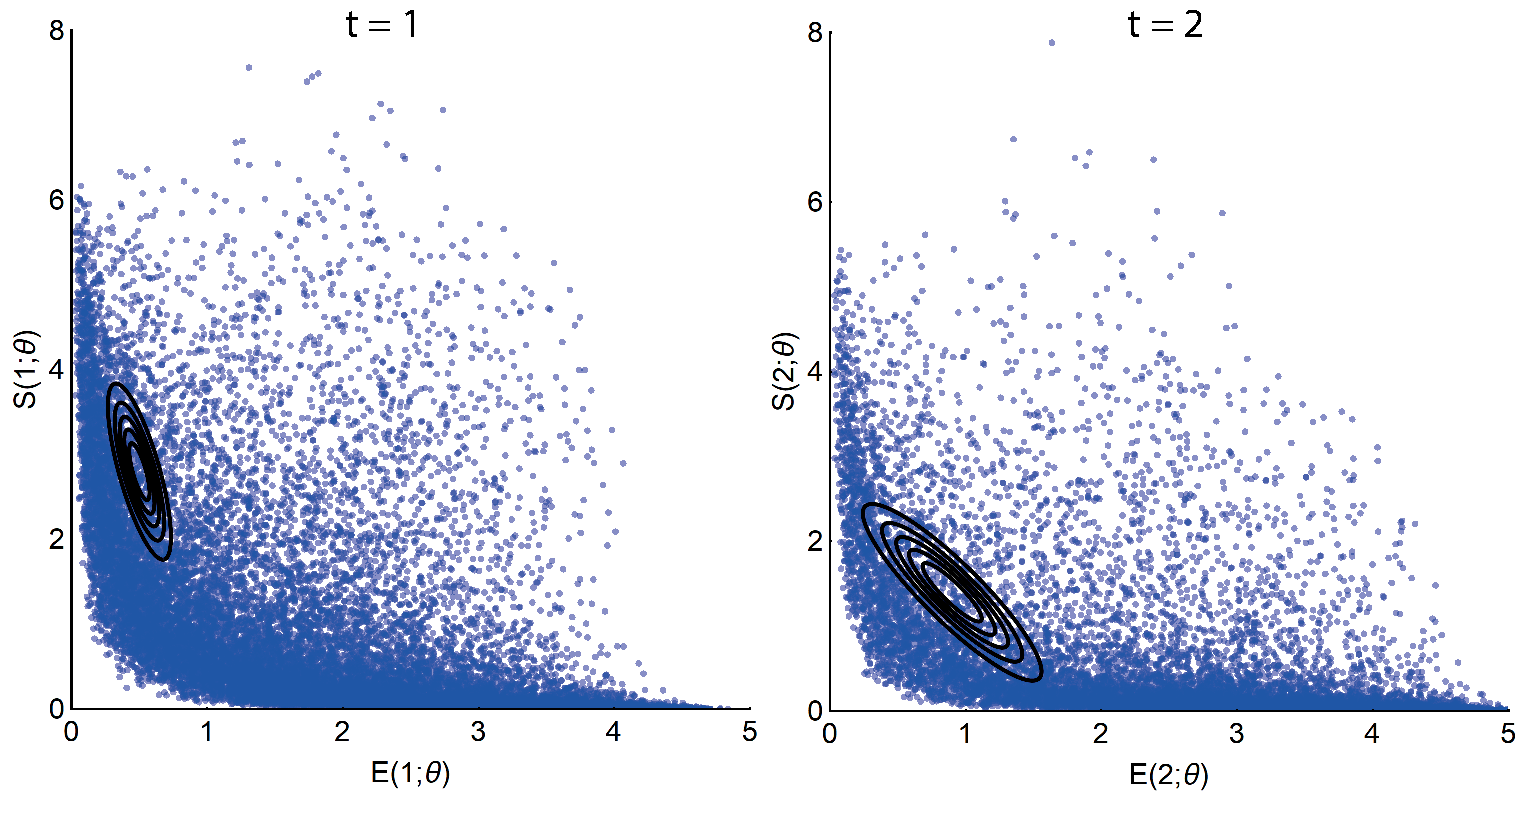
\includegraphics[width=\textwidth]{../figures/mm_4d_main.pdf}}
\caption{\textbf{Output functionals (blue points) $(q_1,q_2)$ (left panel) and $(q_3,q_4)$ (right panel) obtained by independently sampling the priors $p(\boldsymbol{\theta} | \Xi)$ of the 7 parameter Michaelis-Menten model versus the target distribution (black solid contours).} We show 20,000 output samples, where each set of four measurements was obtained from a single sample of the 7 parameters. The output target distribution shown by the contours corresponds to the marginal densities of each pair of enzyme-substrate measurements given by eq. (\ref{eq:MM_4d_output}).}
\label{fig:mm_4d_main}
\end{figure}

Figure \ref{fig:mm_4d_outputs} plots the output samples of enzyme and substrate from the last step of CMC for $t=1$ (blue points) and $t=2$ (orange points) versus the contours (black lines) of the joint marginal distributions of eq. (\ref{eq:MM_4d_output}). The distribution of paired enzyme-substrate samples illustrates that the CMC output samples approximated the target density, itself representing dynamic evolution of the covariance between enzyme and substrate measurements. The target marginal distributions (solid lines) along with their approximations from kernel density estimation (dashed lines) are also shown above and beside the main panel of Figure \ref{fig:mm_4d_outputs}, and largely indicate correspondence.

\begin{figure}[H]
\centerline{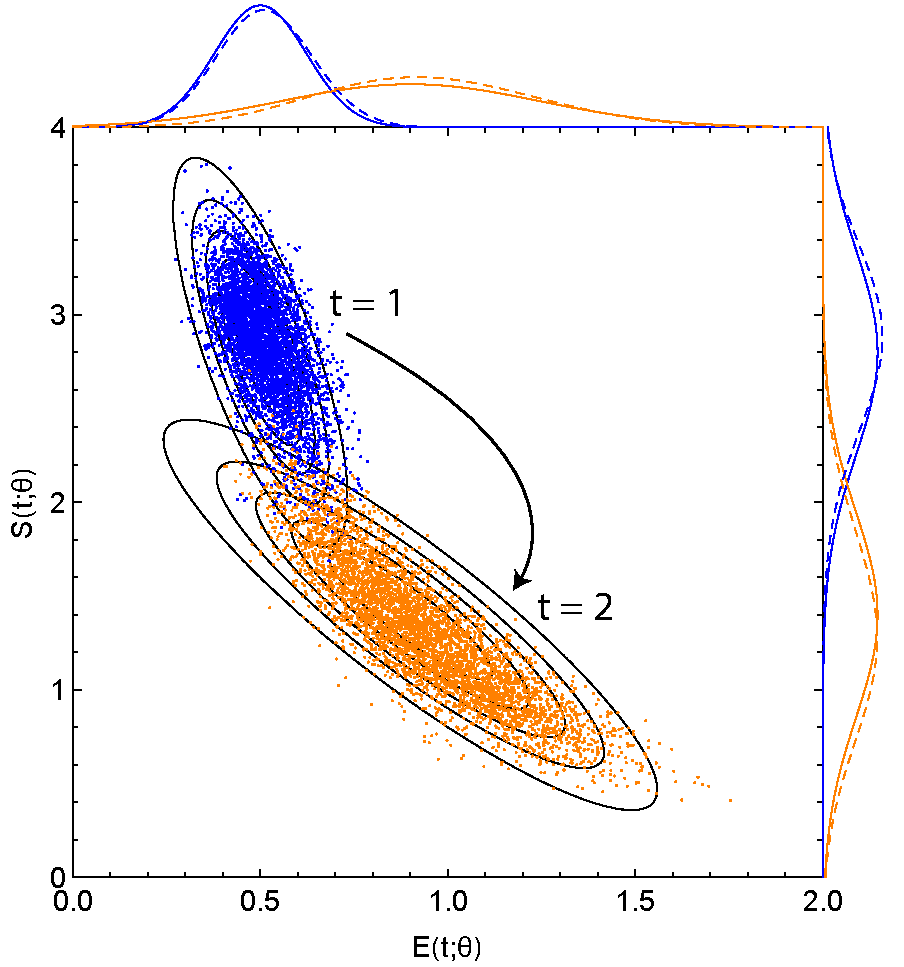
\includegraphics[width=0.65\textwidth]{../figures/mm_4d_outputs.pdf}}
\caption{\textbf{Posterior output samples from CMC (coloured points) versus the contour plots of the joint marginal distributions of eq. (\ref{eq:MM_4d_output}) (black solid lines).} Output functionals for $(q_1,q_2)$ and $(q_3,q_4)$ are given by blue and orange points, respectively. Enzyme and substrate measurements are given by the horizontal and vertical axes, respectively. The solid and dashed coloured lines outside of the panels indicate the true target marginals of eq. (\ref{eq:MM_4d_output}) and those estimated from CMC, respectively. In the ``ContourVolumeEstimator'' step 200,000 independent samples were used and 10,000 samples across each of 4 Markov chains were used in the MCMC step, with the first half of the chains discarded as ``warm-up'' \cite{lambert2018Student}. Mathematica's ``SmoothKernelDistribution'' function with Gaussian kernels \cite{mathematica} of bandwidths varying from 0.1 to 0.4 for the reconstructed marginal densities.}
\label{fig:mm_4d_outputs}
\end{figure}


\subsection{TNF signalling pathway}
We now illustrate how CMC can be applied to an ODE system of larger size, the tumour necrosis factor (TNF) signalling pathway model introduced in \cite{chaves2008bistable} and used by \cite{hasenauer2011identification} to illustrate a Bayesian approach to cell population variability estimation. The model incorporates known activating and inhibitory interactions between four key species within the TNF pathway: active caspase 8 ($x_1$) and active caspase 3 ($x_2$), a nuclear transcription factor ($x_3$) and its inhibitor ($x_4$),
%
\begin{equation}\label{eq:tnf}
\begin{aligned}
\frac{dx_1}{dt} &= -x_1(t) + \frac{1}{2}\left(\beta_4(x_3(t))\alpha_1(u(t)) + \alpha_3(x_2(t))\right)\\
\frac{dx_2}{dt} &= -x_2(t) + \alpha_2(x_1(t)) \beta_3(x_3(t))\\
\frac{dx_3}{dt} &= -x_3(t) + \beta_2(x_2(t)) \beta_5(x_4(t))\\
\frac{dx_4}{dt} &= -x_4(t) + \frac{1}{2}\left(\beta_1(u(t)) + \alpha_4(x_3(t))\right),
\end{aligned}
\end{equation}
%
with initial conditions,
\begin{equation}
x_1(0)=0.0, \quad x_2(0)=0.0, \quad x_3(0)=0.29, \quad x_4(0)=0.625,
\end{equation}
which correspond to the steady state of the system when $x_2=0$. The functions $\alpha_i$ and $\beta_j$ represent activating and inhibitory interactions respectively,
%
\begin{equation}
\begin{aligned}
\alpha_i(z) &= \frac{z^2}{a_i^2 + z^2}, \quad i=1, \dots, 4,\\
\beta_j(z)  &= \frac{b_j^2}{b_j^2 + z^2}, \quad j = 1, \dots, 5,
\end{aligned}
\end{equation}
%
and the parameters $a_i$ for $i\in(1,2,3,4)$ and $b_j$ for $j\in(1,2,3,4,5)$ represent activation and inhibition thresholds. The function $u(t)$ represents a TNF stimulus represented by a top hat function,
%
\begin{equation}
u(t)=\begin{cases}
1, & \text{if $t\in[0,2]$}.\\
0, & \text{otherwise}.
\end{cases}
\end{equation}
%
When there are fewer output measurements than parameters, models tend to be underdetermined meaning that many combinations of parameters can lead to the same combination of output values. A consequence of this unidentifiability is that we cannot perform ``full circle'' inference: that is, using a known parameter distribution to generate an output distribution does not result in that parameter distribution being recapitulated through inference. We illustrate this idea by generating an output distribution by varying a single parameter value between runs of the forward model corresponding to the solution of eq. (\ref{eq:tnf}) and performing inference on all nine system parameters, whilst collecting only two output measurements. Specifically, we vary $a_1\sim \mathcal{N}(0.6, 0.05)$, whilst holding the other parameters constant, $$(a_2,a_3,a_4,b_1,b_2,b_3,b_4,b_5)=(0.2, 0.2, 0.5, 0.4, 0.7, 0.3, 0.5, 0.4)$$ and measure $q_1=x_1(2.0)$ and $q_2=x_2(1.0)$ for each forward model simulation. In doing so, we obtain an output distribution well-approximated by the bivariate normal distribution,
%
\begin{equation}\label{eq:tnf_circular_target}
\begin{aligned}
\boldsymbol{q} = \begin{pmatrix} q_1 \\ q_2 \end{pmatrix}
&=
\begin{pmatrix}
x_1(2.0)\\
x_2(1.0)\\
\end{pmatrix} \\
&\sim  \mathcal{N}
\begin{bmatrix}
\begin{pmatrix}
0.26\\
0.07\\
\end{pmatrix}, \;\;
\begin{pmatrix}
2.1\times 10^{-4} & 5.9\times 10^{-5}\\
5.9\times 10^{-5} & 1.8\times 10^{-5}\\
\end{pmatrix}
\end{bmatrix}.
\end{aligned}
\end{equation}
%
We now apply CMC to the target output distribution given by eq. (\ref{eq:tnf_circular_target}) to estimate a posterior distribution over all nine parameters of eq. (\ref{eq:tnf}). Apart than for a few cases, the priors for each parameter were chosen to \emph{exclude} the values that were used to generate the output distribution (see Table \ref{tab:priors}), to illustrate the non-equivalence between the recovered posterior distribution and the data generating process. In Figure \ref{fig:tnf_circular_versus}A, we plot the actual parameter values (horizontal axis) used in the true data generating process versus the inferred values (vertical axis). This illustrates that apart from $a_1$, where the estimated parameter values correspond well with the range of values used to generate the data, due to the choice of priors there is a disjunction between the actual and estimated values. Despite these differences, due to the model being underdetermined, it is nonetheless possible to use CMC to sample from an output distribution that well approximates the target (Figure \ref{fig:tnf_circular_versus}B).


\begin{figure}[H]
\centerline{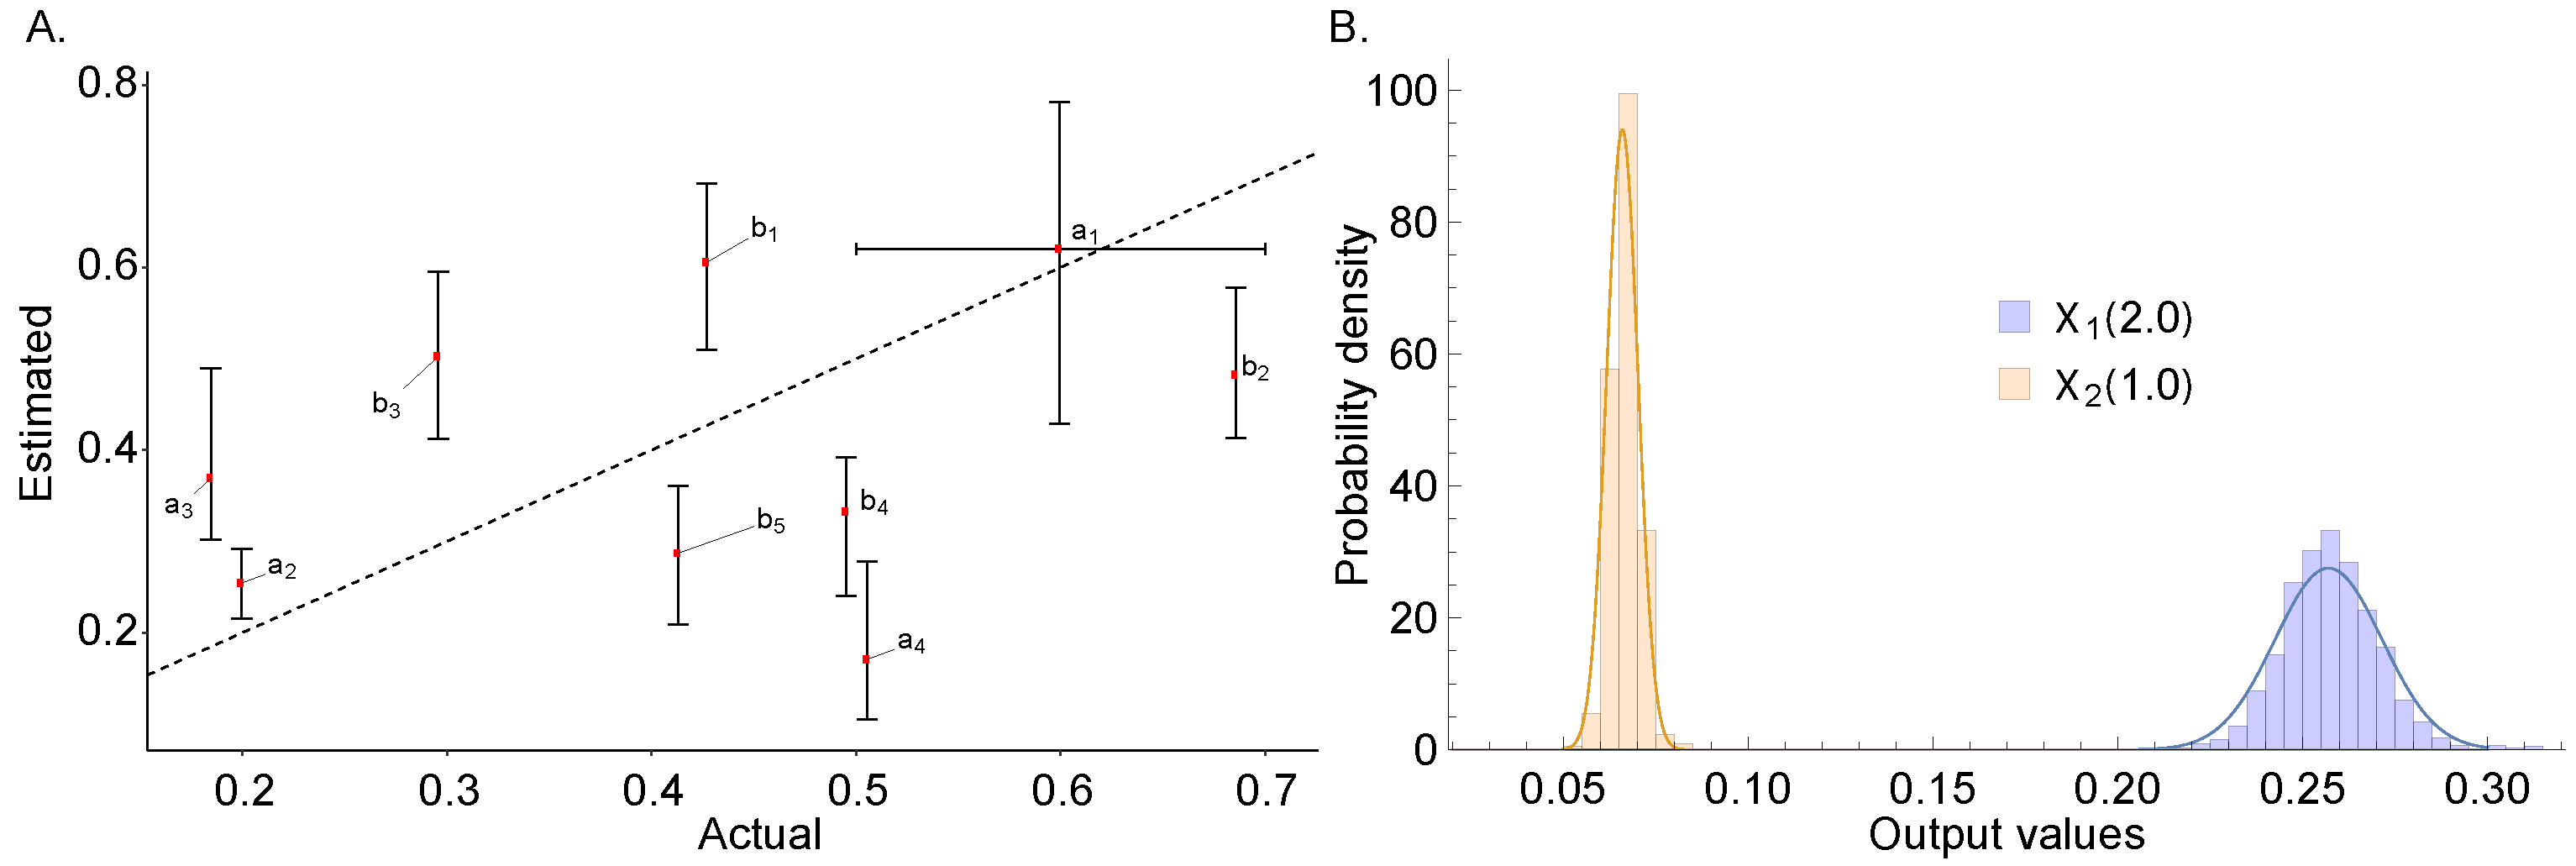
\includegraphics[width=1.5\textwidth]{../figures/tnf_circular_both.pdf}}
\caption{\textbf{(A) actual parameter values versus estimated quantiles for the output distribution for the TNF signalling pathway model with output distribution given and (B) the marginal output target (solid lines) given by eq. (\ref{eq:tnf_circular_target}) and sampled output distribution (histograms).} In A, in the vertical direction, red points indicate 50\% posterior quantiles and upper and lower whiskers indicate 97.5\% and 2.5\% quantiles, respectively; in the horizontal direction, with the exception of $a_1$, red points indicate the parameter values used to generate the data; for $a_1$ the red point indicates the mean of the normal distribution used to generate the data and the whiskers indicate its 95\% quantiles. In CMC, 10,000 independent samples were used in the ``ContourVolumeEstimator'' step and 5,000 MCMC samples across each of 4 Markov chains were used in the second step, with the first half of the chains discarded as ``warm-up'' \cite{lambert2018Student}.}
	\label{fig:tnf_circular_versus}
\end{figure}

Cell populations may be well described by subpopulations which each evolve along characteristic trajectories over time. We now apply CMC to investigate a bimodal output distribution for the TNF signalling pathway model similar to that investigated by \cite{hasenauer2011identification}. In particular, we aim to find a distribution over parameter values which, when used as inputs to the solution to the ODE system, results in the following output distribution,
%
\begin{equation}
\boldsymbol{q} = \begin{pmatrix} q_1 \\ q_2 \\ q_3 \end{pmatrix},
\end{equation}
where,
\begin{equation}
\begin{aligned}
q_1 = \boldsymbol{x}_2(1.0) &\sim \mathcal{N}(0.06, 0.01)\\
q_2 = \boldsymbol{x}_2(2.0) &\sim\frac{1}{2}\left(\mathcal{N}(0.1, 0.01) + \mathcal{N}(0.14, 0.01)\right)\\
q_3 = \boldsymbol{x}_2(4.0) &\sim\frac{1}{2}\left(\mathcal{N}(0.1, 0.01) + \mathcal{N}(0.20, 0.01)\right),\\
\end{aligned}
\end{equation}
%
where the target distributions for $\boldsymbol{q}_2(2.0)$ and $\boldsymbol{q}_2(4.0)$ indicate mixtures of univariate normals, and the priors used are described in Table \ref{tab:priors}. This target distribution, along with the unique trajectories obtained by applying the CMC algorithm for 5,000 MCMC steps, are shown in Figure \ref{fig:tnf_samples_vs_distribution}. This figure illustrates that given by bimodality of the output distribution, CMC estimates a corresponding subpopulation structure in the parameter distribution without \textit{a priori} specification of the number of clusters.

\begin{figure}[H]
	\centerline{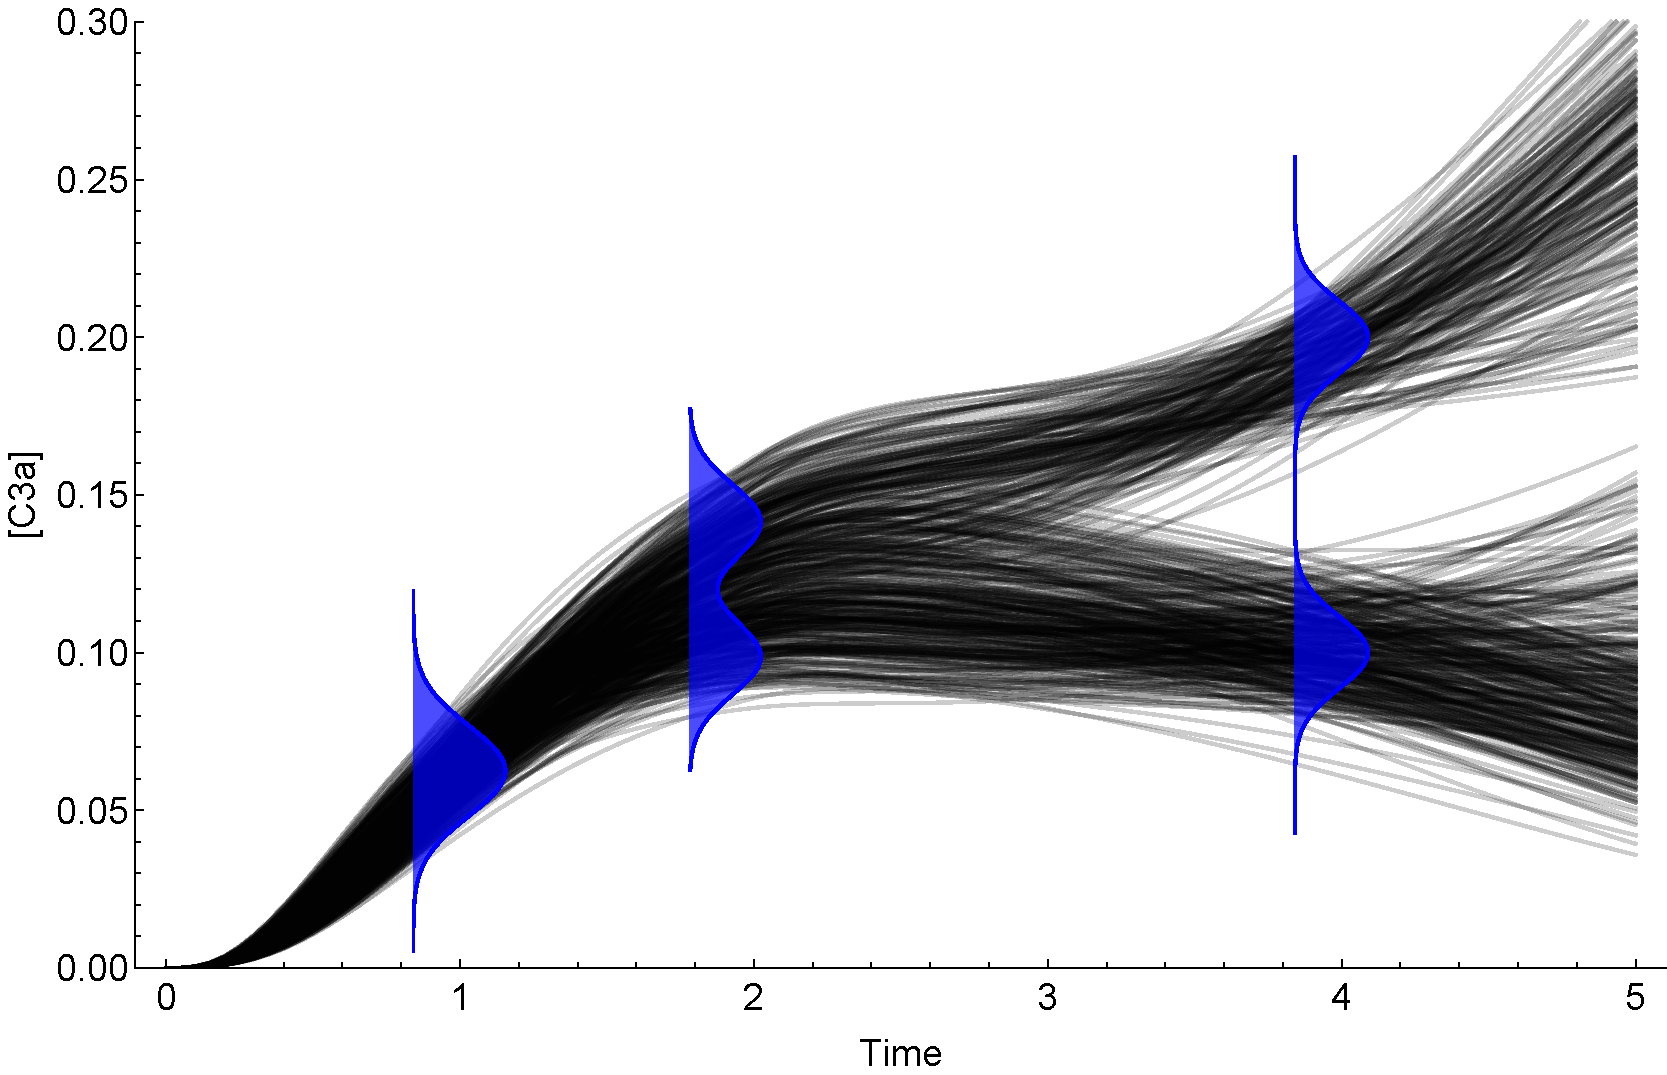
\includegraphics[width=0.8\textwidth]{../figures/tnf_samples_vs_distribution.pdf}}
	\caption{\textbf{The target output distribution (dashed plots with grey filling) and unique trajectories (black solid lines) obtained from the posterior parameter distribution.} In CMC, 10,000 independent samples were used in the ``ContourVolumeEstimator'' step and 5,000 MCMC samples across each of 4 Markov chains were used in the second step, with the first half of the chains discarded as ``warm-up'' \cite{lambert2018Student}.}
	\label{fig:tnf_samples_vs_distribution}
\end{figure}

\begin{table}[H]
\centering
%\scriptsize
\begin{adjustwidth}{0in}{0in}%
\begin{tabularx}{1.0\textwidth}{llclcc}
Model	& Target  & Parameter & Prior    & Prior  & Prior  \\
        & density &           & density  & $p_1$  & $p_2$  \\
\toprule
Growth  & 2D     & $R_T$       & uniform & $2.5 \times 10^5$ &  $8 \times 10^5$\\
factor  & normal & $k_1$       & uniform & 0.25 & 3.0\\
                && $k_{-1}$    & uniform & 2.0 & 20.0\\
                && $k_{deg}$   & uniform & 0.005 & 0.03\\
                && $k^*_{deg}$ & uniform & 0.1 & 0.5\\
\toprule
Growth  & 2D     & $R_T$ & normal & $5 \times 10^5$ &  $1 \times 10^5$\\
factor  & normal & $k_1$ & normal & 0.5 & 0.1\\
                && $k_{-1}$ & normal & 3.0 & 1.0\\
                && $k_{deg}$ & normal & 0.02 & 0.005\\
                && $k^*_{deg}$ & normal & 0.3 & 0.1\\
\toprule
Michaelis- & bimodal  & $k_f$ & uniform & 0.2 &  15\\
Menten     & normal   & $k_r$ & uniform & 0.2 & 2.0\\
&& $k_{cat}$ & uniform & 0.5 & 3.0\\
\toprule
Michaelis- & 4D    & $k_f$ & uniform & 0.2 &  15\\
Menten     & normal& $k_r$ & uniform & 0.2 & 2.0\\
&& $k_{cat}$ & uniform & 0.2 & 3.0\\
&& $E_0$ & uniform & 3.0 & 5.0\\
&& $S_0$ & uniform & 5.0 & 10.0\\
&& $C_0$ & uniform & 0.0 & 0.2\\
&& $P_0$ & uniform & 0.0 & 0.2\\
\toprule
TNF & bivariate & $a_1$ & uniform & 0.4 & 0.8\\
signalling & normal& $a_2$ & uniform & 0.1 & 0.7\\
&& $a_3$ & uniform & 0.3 & 0.7\\
&& $a_4$ & uniform & 0.1 & 0.3\\
&& $b_1$ & uniform & 0.5 & 0.7\\
&& $b_2$ & uniform & 0.4 & 0.6\\
&& $b_3$ & uniform & 0.4 & 0.6\\
&& $b_4$ & uniform & 0.2 & 0.4\\
&& $b_5$ & uniform & 0.2 & 0.4\\
\toprule
TNF  & bimodal  & $a_1$ & uniform & 0.5 & 0.7\\
signalling& normal & $a_2$ & uniform & 0.1 & 0.3\\
&& $a_3$ & uniform & 0.1 & 0.3\\
&& $a_4$ & uniform & 0.4 & 0.6\\
&& $b_1$ & uniform & 0.3 & 0.5\\
&& $b_2$ & uniform & 0.6 & 0.8\\
&& $b_3$ & uniform & 0.2 & 0.4\\
&& $b_4$ & uniform & 0.4 & 0.6\\
&& $b_5$ & uniform & 0.3 & 0.5\\
\end{tabularx}
\caption{\textbf{The priors used for each problem in \S\ref{sec:results}.} The parameters $p_1$ and $p_2$ indicate the prior hyperparameters: for uniform priors, these correspond to the lower and upper limits; for normal priors, they correspond to the mean and standard deviation.}
\label{tab:priors}
\end{adjustwidth}
\end{table}

\section{Discussion}
\label{sec:discussion}
Determining the cause of variability in cellular processes is crucial in many applications, ranging from bioengineering to drug development. In this paper, we introduce a Bayesian method for estimating cellular heterogeneity from ``snapshot'' measurements of cellular properties, taken at discrete intervals throughout the experimental course. Our approach assumes what we term a ``heterogeneous ordinary differential equation'' (HODE) framework, in which biochemical processes in individual cells are assumed to follow dynamics governed by a common ODE, although with idiosyncratic differences in parameter values. In this framework, estimating heterogeneity in cellular processes amounts to determining the probability distributions over parameter values of the governing ODE. Our method of estimation is a two-step Monte Carlo sampling process we term ``Contour Monte Carlo'' (CMC) which does not require \textit{a priori} specification of cell population substructure unlike other approaches. CMC can be used to process high volumes of individual cellular measurements since the framework involves fitting a kernel density estimator to raw experimental data and using these distributions rather than data as the target outcome. CMC also allows for arbitrary multivariate structure in the measurement space, meaning it can capture correlations that occur between the same cellular species at different timepoints or, for example, contemporaneous correlations between different cellular compartments. Being a Bayesian approach, CMC uses prior distributions over parameter values to ensure uniqueness of the posterior distribution, allowing pre-experimental knowledge to be used to improve estimation robustness. The flexible and robust framework that CMC provides means it can be used to perform automatic inference for wide-ranging systems of practical interest.

Our approach also provides a natural way to test that the process is working satisfactorily. Feeding the posterior parameter samples obtained by CMC into forward model simulations, results in a distribution over output values that can be compared to the target. Indeed, we have found this comparison indispensable in applying CMC in practice and include it as the last step in the CMC algorithm (Algorithm \ref{alg:cmc}). Discrepancies between the target output distribution and samples from it by CMC can occur either as a result of poor estimates of the ``contour volume distribution'' in the first stage of the algorithm or due to insufficient MCMC samples in the second. Either of these issues can often be easily addressed and although kernel density estimation in high dimensional spaces remains an open research problem, we have found vine copula kernel density estimation works well for the dimensionality of output measurements we investigate here \cite{nagler2016evading}.

Failure to reproduce a given output distribution can also indicate that the generating model (the priors and the forward model) are incongruent with experimental results. This may either be due to misspecification of the ODE system or, that our assumption the process is deterministic is inappropriate. Our approach currently assumes that output variation is dominated by cellular variation in the parameter values of the underlying ODE, with measurement noise making a negligible contribution. Whether this is a reasonable assumption depends on the system under investigation and, more importantly, on experimental details. We recognise that neglecting measurement noise when it is an important determinant of the observed data means CMC will overstate cellular variation. It may also mean that some output distributions cannot be obtained by our model system (the HODEs without noise). Future work allowing inclusion of a stochastic noise process or, more generally, including stochastic cellular mechanisms is thus likely to be worthwhile.

Whilst we have labelled the approach we follow here as Bayesian, since it involves explicit estimation of probability distributions and involves priors over parameter values, we recognise that it is not in the form typically utilised by exponents of this framework. This is because rather than aiming to formulate a model that describes output observations, our approach aims to recapitulate output \emph{distributions}. Others \cite{BJW-18}, (including us \cite{lambert2018inverse}), have considered similar problems before; perhaps most notably by Albert Tarantola in his landmark work on inverse problem theory (see, for example, \cite{tarantola2005inverse}), which has generated considerable interest in areas such as the geosciences \cite{mosegaard1995monte,vukicevic2008analysis}. In Tarantola's framework, a joint input parameter and output space is considered, where prior knowledge and experimental theory combine elegantly to produce a posterior distribution whose marginal output distribution is a weighted ``conjunction'' of various sources of measurement. %Whilst we believe the inverse problems covered by the Tarantola framework are different to ours (Tarantola combines parameter-output measurement distributions via ``conjunctions'' whereas we use push-forward measures resulting from inputting parameter values into the forward map), there are equivalences between the two frameworks. This work has seen considerable interest in areas such as the geosciences \cite{mosegaard1995monte,vukicevic2008analysis}, and we propose that Tarantola's approach may prove useful for the biosciences. %In particular, we posit that this approach provides a single framework for generalised Bayesian inference that encompasses either output data or output distributions as outcome measures.
%SJT -- This is the first mention of push forward measures, which I feel is too dangerous. 


The natural world is rife with variation. Mathematical models represent frameworks for understanding the causes of such variation. Typically, the state of biological knowledge is such that one effect, a given pattern of variation, has many possible causes, and observational or experimental data are necessary to apportion weight to each of them, in a process which amounts to solving an inverse problem. The approach we describe here follows the Bayesian paradigm of inverse problem solving whereby uncertainty in potential causes is reflected by probability distributions. Here, we illustrate the utility of our method by applying it to estimate cellular heterogeneity in biochemical processes however, it could equally be used to understand the inversion of systems modeled by an undeterdetermined input to output map in the form of an algebraic map, or a system of odes or pdes, arising in other areas. %Whilst describing the inversion process of deterministic models using probability distributions may sound contradictory, it is worth acknowledging that many ODE systems are structurally unidentified meaning there is irreducible uncertainty over some regions of parameter space.
Contour Monte Carlo provides an automatic framework for performing inference on such underdetermined systems and the use of priors allows for robust and precise parameter estimation unattainable through the data alone.




\section{Author contributions}
BL, DJG and SJT conceived the study. BL carried out the analysis. All authors helped to write and edit the manuscript.


\nolinenumbers

\bibliographystyle{unsrt}
\bibliography{Bayes}
\end{document}

